\clearpage
\appendix
\section{Technical Appendices and Supplementary Material}
\noindent This Supplementary Material is organized as follows.  

\begin{itemize}[left=0pt]
    \item In \Cref{sec:Exp_Details}, we provide the training details of \model, including initialization (\Cref{sec:init_Details}), training procedures (\Cref{sec:tra_Details}), and multi-image training strategy(\Cref{sub:multi_init_Details}).
    \item In \Cref{sup:t2i}, we show quantitative evaluations of our method on text-to-image generation benchmarks.
    \item In \Cref{sec:data_const}, we detail our data construction pipeline and the dataset details used across the two-stage training.
    \item In \Cref{sec:Experiment_Details}, we elaborate on the experimental setup, including datasets and metrics (\Cref{sec:Benchmark_Details}), as well as detailed descriptions of baseline methods(\Cref{sec:Baselines_Details}).
    \item In \Cref{sec:Qualitative_Study}, we present qualitative results that demonstrate the capabilities of \model in various settings, such as image reconstruction(\Cref{sec:Reconstruction}), segmentation(\Cref{sec:Segmentation}), multi-image generation(\Cref{sec:Multi-Image}), and in-context image generation(\Cref{sec:mmicl}).
    \item In \Cref{app:applications}, we demonstrate the versatility of \model across diverse multimodal generation tasks, including segmentation, subject-driven generation, and multimodal in-context learning.
    \item In \Cref{app:limitation}, we discuss the current limitations of our method, such as its dependence on autoregressive generators, generation fidelity, and safety considerations.
\end{itemize}


\section{Training Details}
\label{sec:Exp_Details}

\subsection{Initialization Details}
\label{sec:init_Details}

The multimodal encoder is initialized using the vision encoder from CLIP-Large-Patch14~\citep{Radford2021LearningTV}, with an image receptive field of $224 \times 224$, and the FlanT5-XL encoder~\citep{flant5}, with a context length of 512 tokens. This encoder converts each image into 256 tokens for use as context in the generator.

To implement the MLP-based projection, we train the MLP projector on the LLaVA-CC3M-Pretrain-595K dataset~\citep{liu2023llava}, following the alignment training setup used by LLaVA. Specifically, we freeze both the vision and text encoders (CLIP-Large-Patch14 and FlanT5-XL, respectively) and train only the MLP layers. The resulting pretrained MLP layers are then directly incorporated into the multimodal encoder of \model.


\begin{figure*}[htbp]
\centering
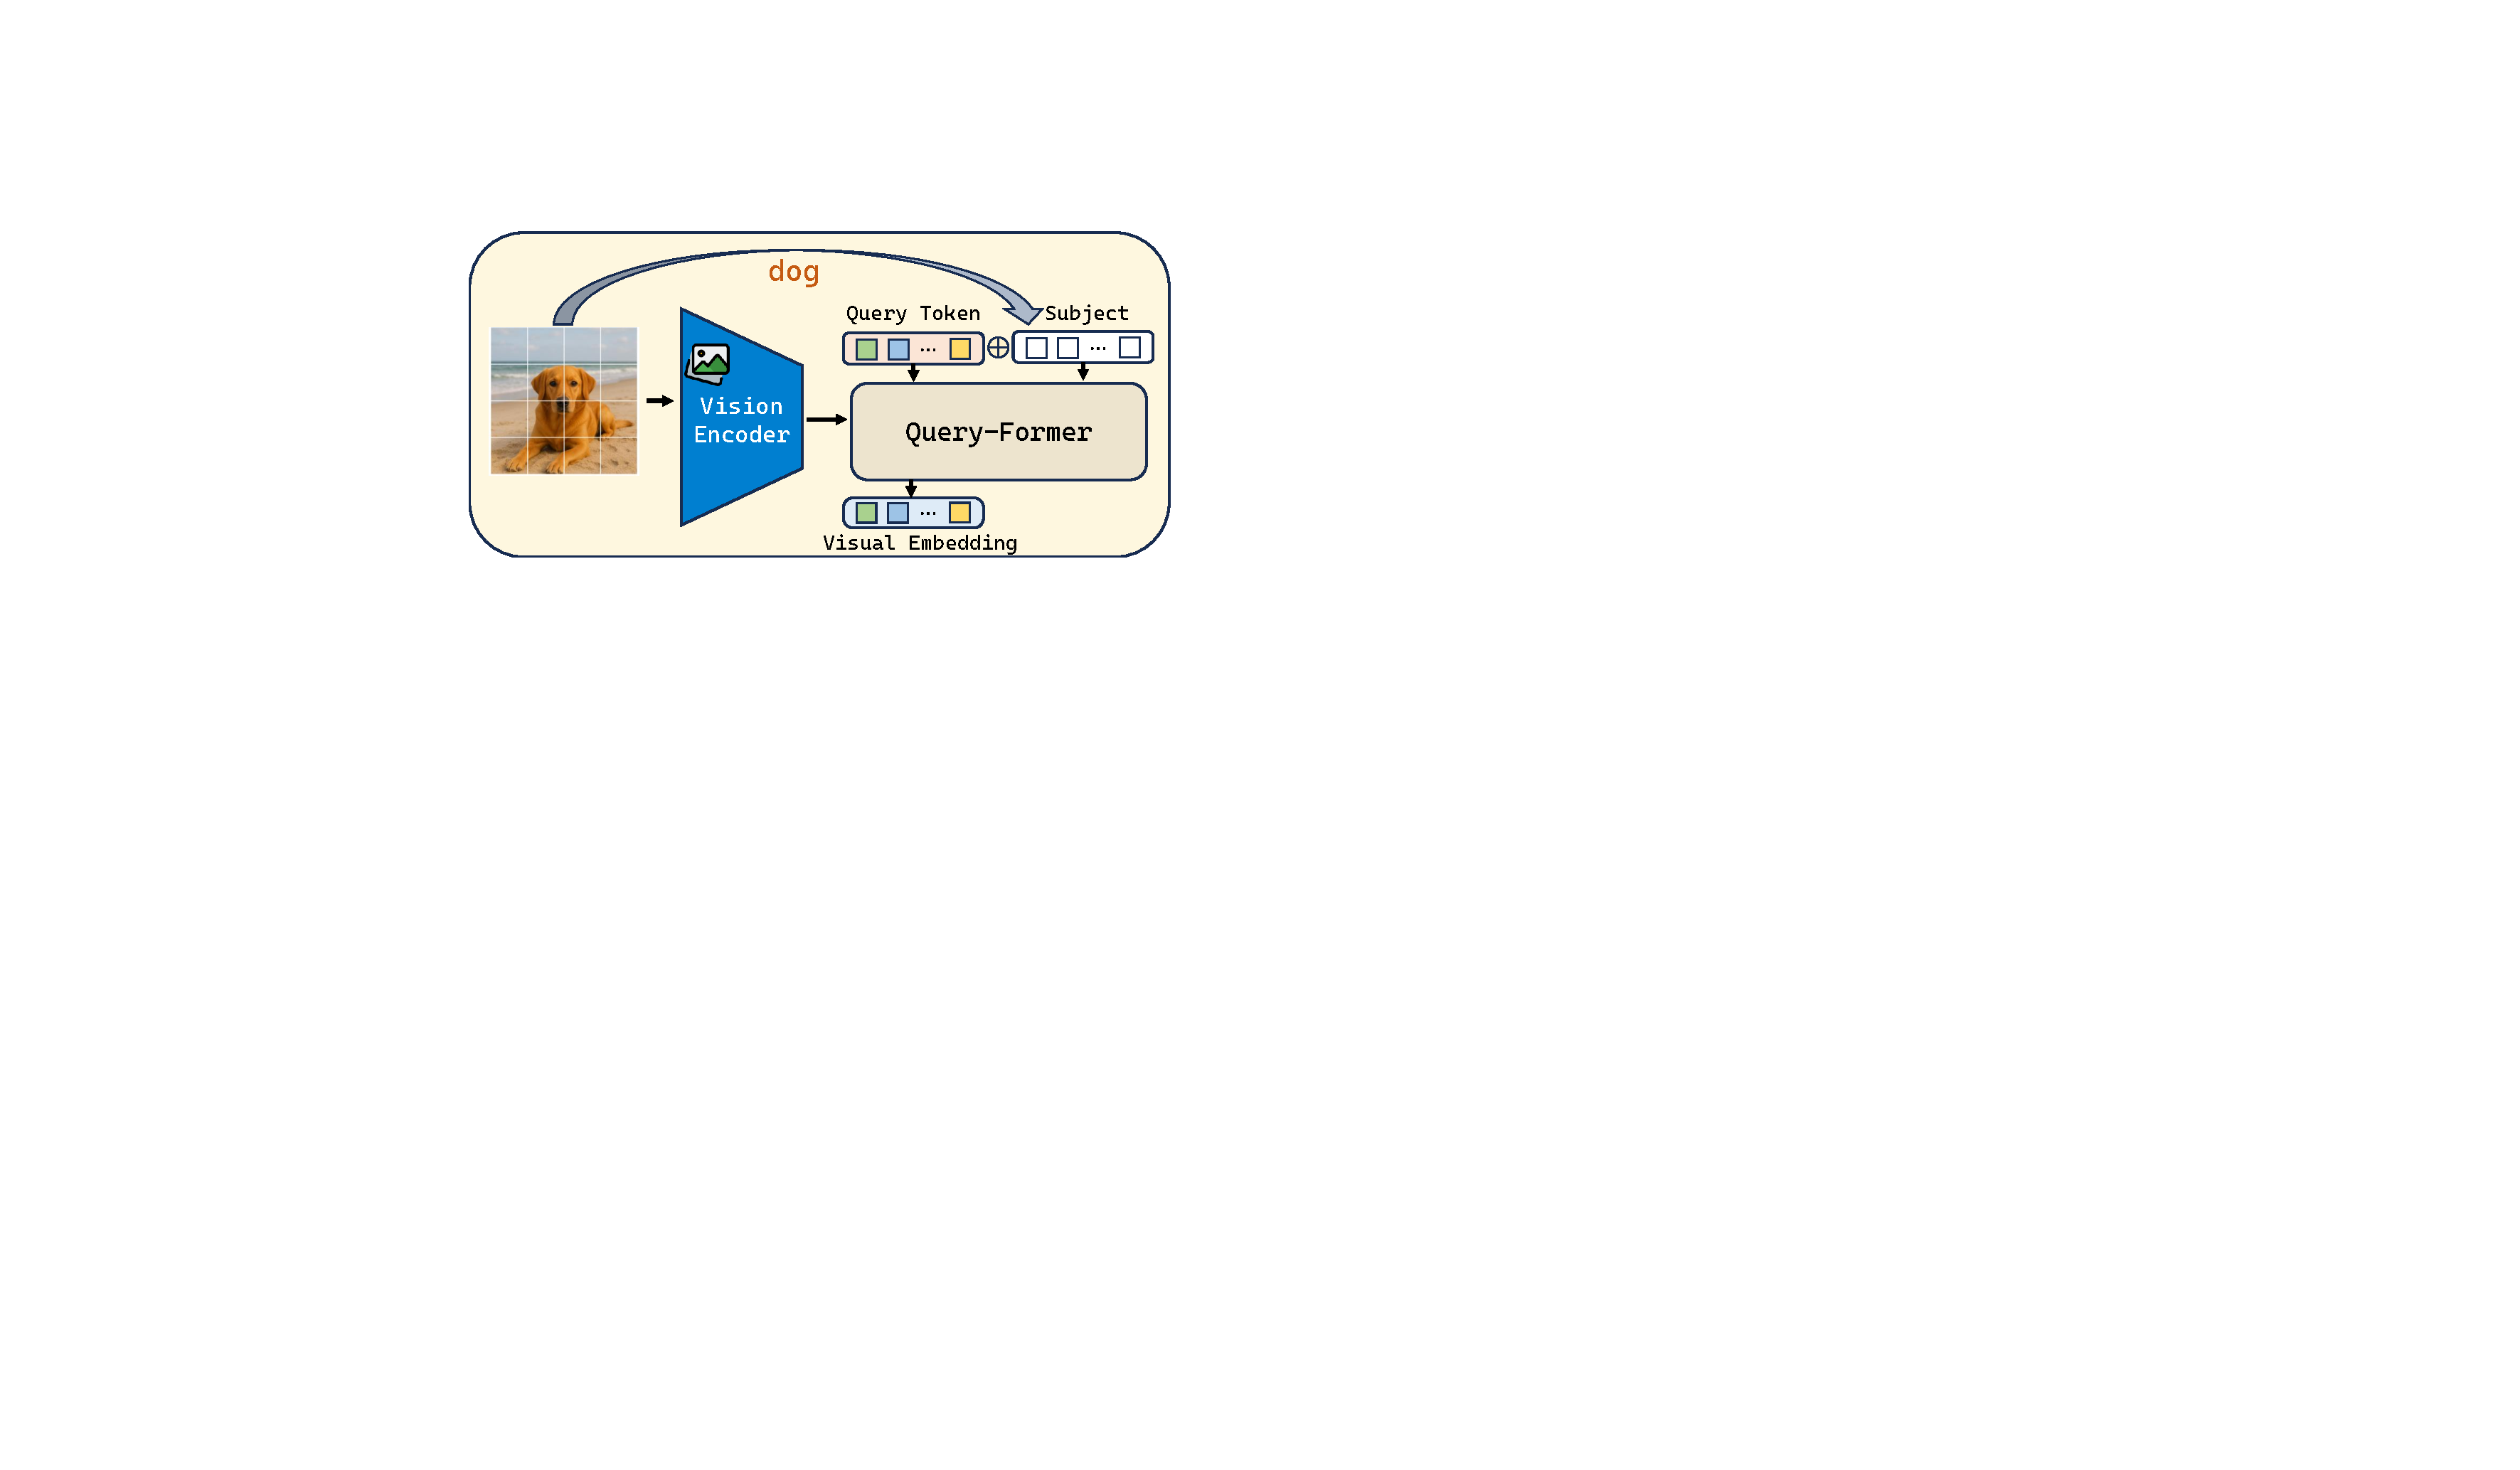
\includegraphics[width=0.8\textwidth]{figures/qformer.pdf}
\caption{Overview of text-guided visual distillation using the Query-based variant of \model.}
\label{fig:qformer}
\end{figure*}

The projector consists of a two-layer MLP with an intermediate dimension of 4,096, employing SiLU activation functions.
The autoregressive generator is initialized from LlamaGen-XL~\citep{llamagen} with 775 million parameters. 
However, the original LlamaGen implementation contains a fundamental error in its 2D Rotary Positional Embedding\citep{lu2023unifiedio2,EVA-02} (ROPE) mechanism\footnote{\url{https://github.com/FoundationVision/LlamaGen/issues/54}}, which leads to a loss of information in the query and key vectors during attention computation. To address this, we correct the ROPE implementation in our code and continue training the revised model on both the Midjourney dataset~\citep{midjourney-niji-1m-llavanext} and the LAION-COCO dataset used in LlamaGen pretraining, effectively replicating the original pretraining conditions. This continued training enables the model to adapt to the corrected ROPE mechanism. The resulting model is then used to initialize our autoregressive generator.

\subsection{Training Procedure}
\label{sec:tra_Details}

The model training comprises two distinct stages:

\textbf{Stage 1}: We freeze the multimodal encoder and train only the projector and generator modules for one epoch, using a global batch size of 128. Optimization employs the Adam optimizer with an initial learning rate of $5 \times 10^{-4}$, a linear warm-up over the initial 5% of steps, and a subsequent cosine decay schedule.

\textbf{Stage 2}: We fine-tune the entire model, excluding the vision encoder, for two epochs. The learning rate is reduced to $1 \times 10^{-4}$, with all other optimization settings remaining consistent with Stage 1. This phase primarily enhances cross-modal interactions and improves conditional image generation capabilities from combined visual and textual inputs.

Training is conducted across 8 NVIDIA A100 GPUs, each equipped with 80 GB memory, taking approximately 1.5 days. Specifically, Stage 1 training involves 2.48 million data points over a single epoch, completed in roughly 14 hours. Stage 2 training utilizes 1.3 million data points over two epochs, taking approximately 20 hours in total.

Ablation studies follow the same training schedule, with one epoch of training on Stage 1 data, followed by two epochs on Stage 2 data.

\subsection{Multi-Image Training}
\label{sub:multi_init_Details}
In \textbf{multi-image training} scenario, the context length of \model is expanded to 1,280 tokens to accommodate up to 4 images per context. For the Query-based variant of \model, token compression techniques enable processing up to 14 images per context with 512 context length.

We utilize 1.5 million multi-image samples, each comprising segmented sub-images accompanied by textual descriptions. The model is trained to reconstruct original images based on these segmented inputs and their corresponding captions. Training incorporates a mixture of Stage 2 data and multi-image samples for an additional epoch.

Qualitative assessments, presented in \Cref{fig:multi}, demonstrate that multi-image training significantly enhances the model's capability to preserve detailed visual information in complex multimodal contexts.

\begin{figure*}[t]
\centering
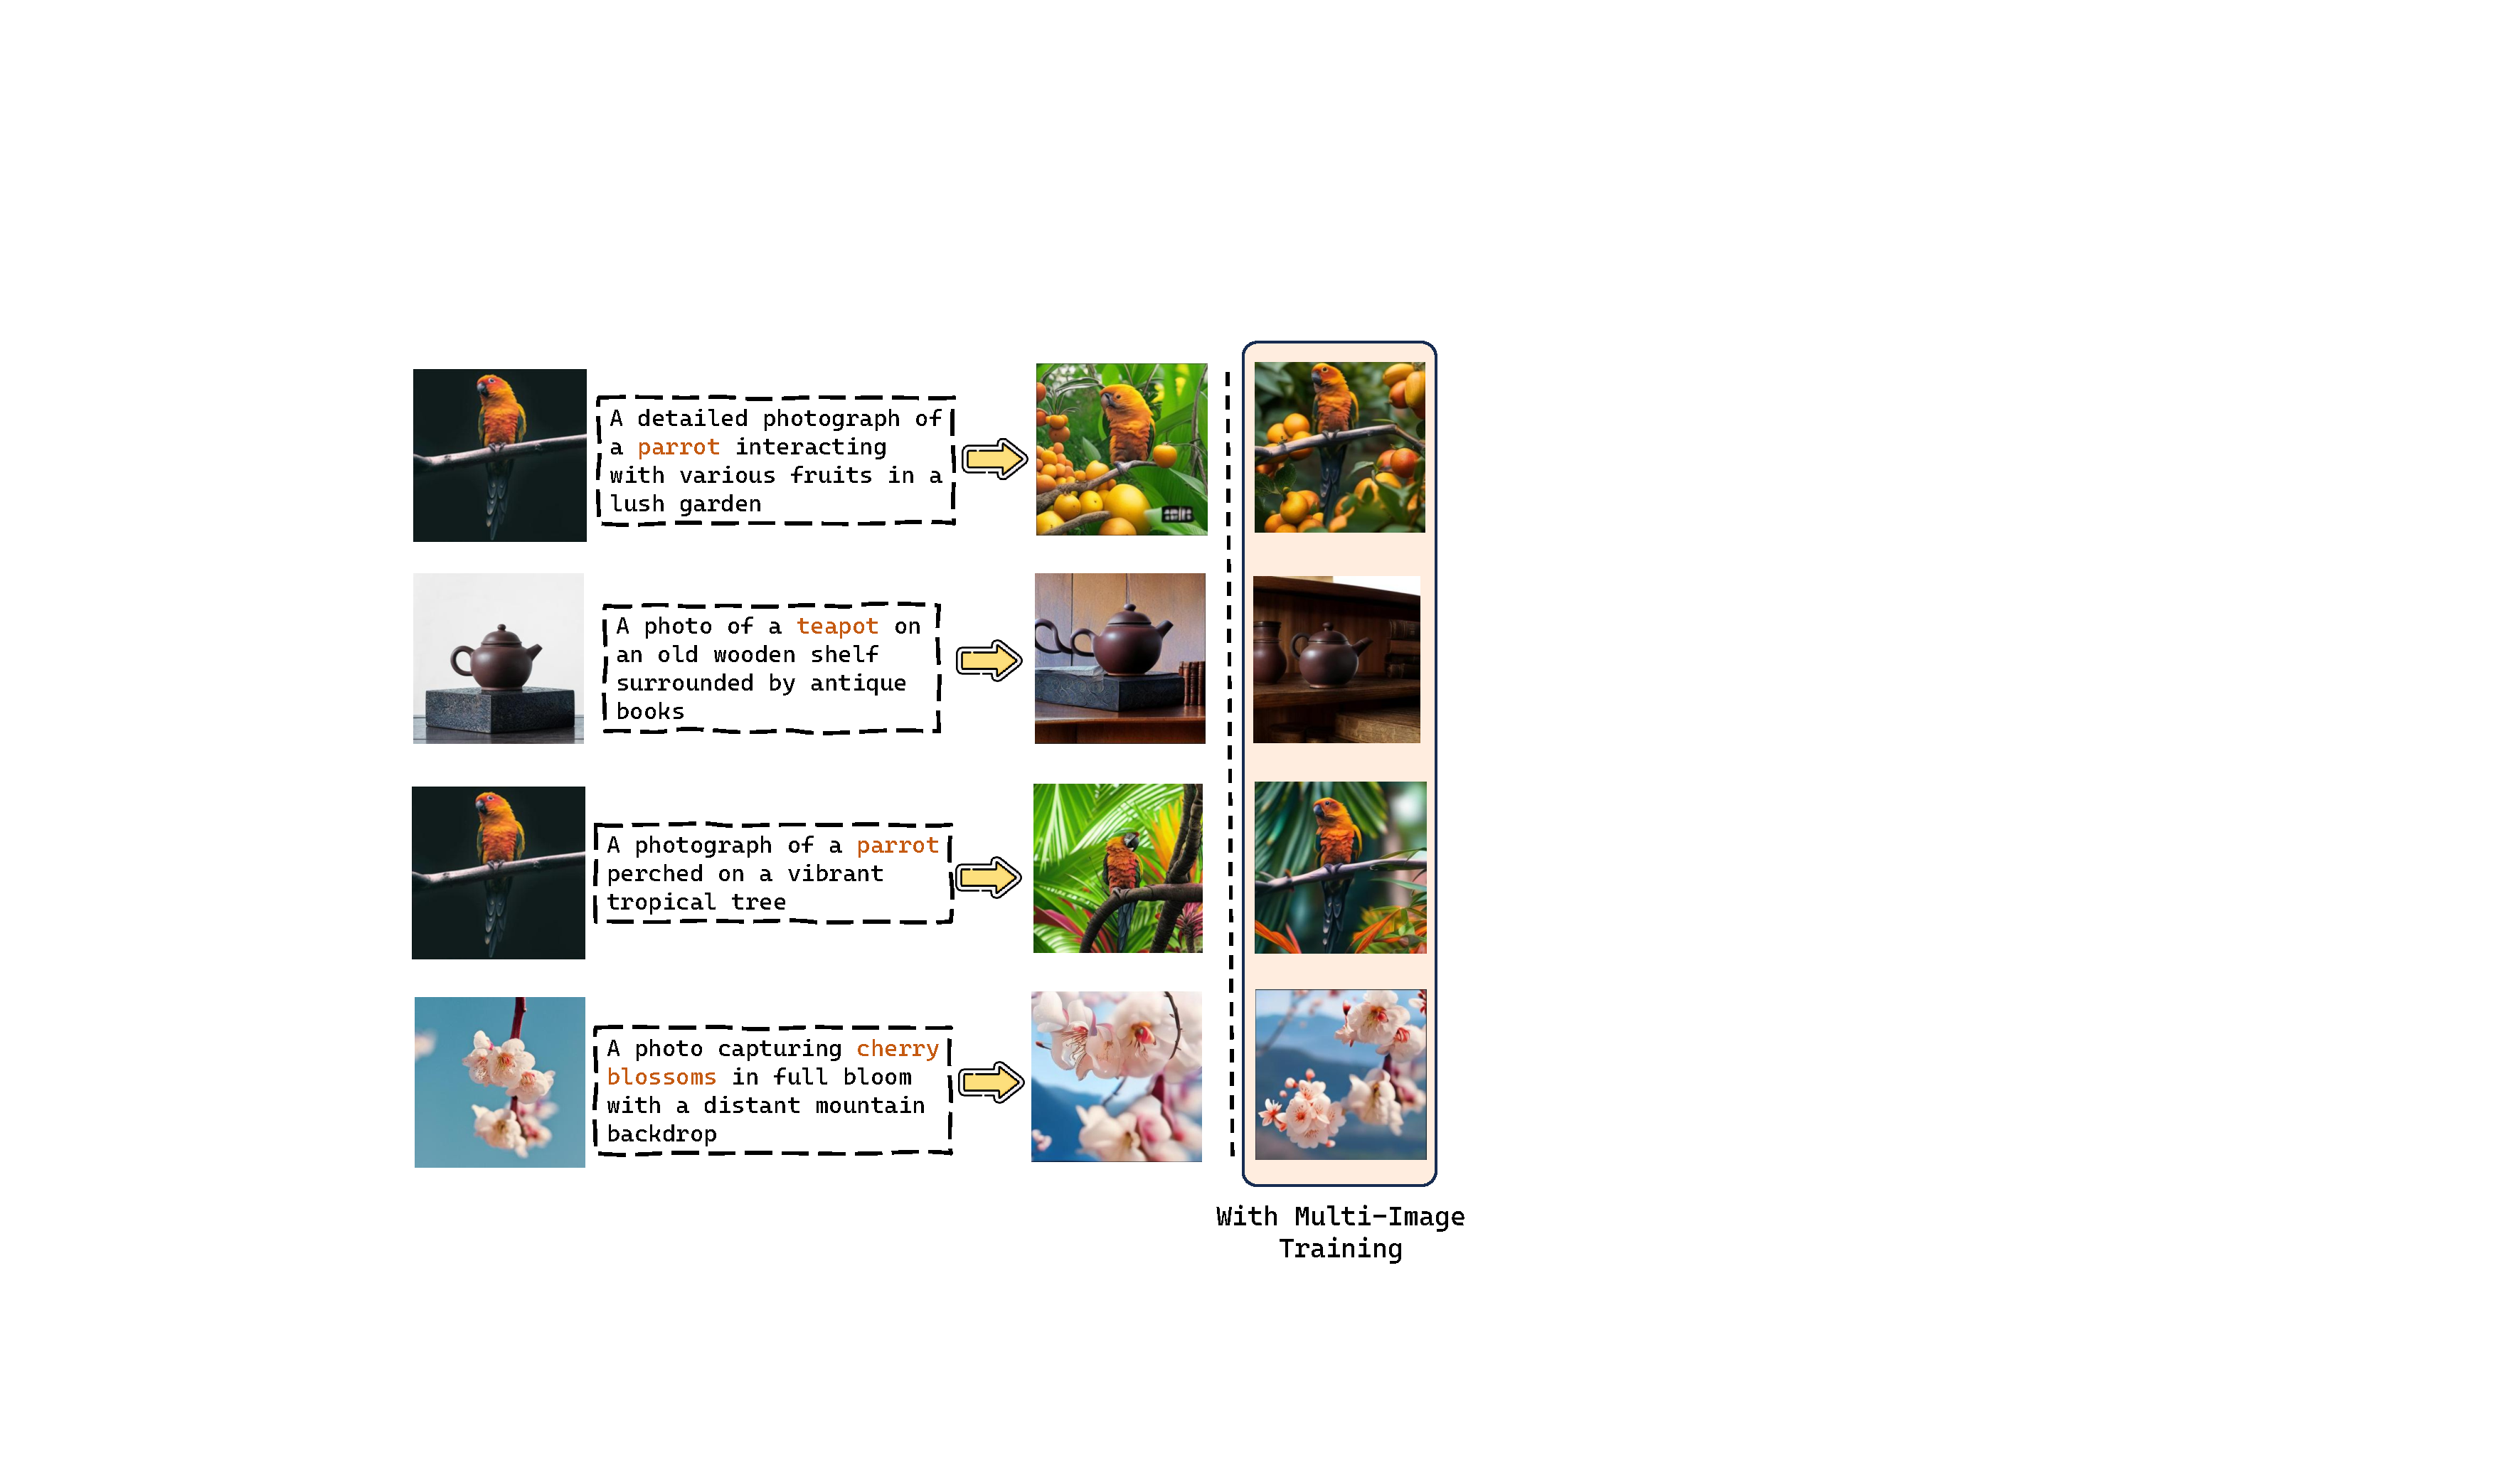
\includegraphics[width=1.0\textwidth]{figures/multi_exp.pdf}
\caption{Qualitative assessment demonstrating improved preservation of visual details by \model following multi-image training.}
\label{fig:multi}
\end{figure*}

\section{Text-to-Image Generation Evaluation}
\label{sup:t2i}
\begin{table*}[t]
    \centering
    \caption{GenEval benchmark results for text-to-image generation, classifying methods as either autoregressive or diffusion-based models. Due to our method's model size and suboptimal generators, we experience poor performance in text-to-image generation.}
    \resizebox{\textwidth}{!}{
    \begin{tabular}{@{}cl
        >{\centering\arraybackslash}m{1.4cm}
        >{\centering\arraybackslash}m{1.4cm}
        >{\centering\arraybackslash}m{1.4cm}
        >{\centering\arraybackslash}m{1.4cm}
        >{\centering\arraybackslash}m{1.4cm}
        >{\centering\arraybackslash}m{1.4cm}
        >{\centering\arraybackslash}m{1.4cm}
        @{}}
        \toprule
         & \textbf{Method} & \textbf{Single Object} & \textbf{Two Object} & \textbf{Counting} & \textbf{Colors} & \textbf{Position} & \textbf{Attribute Binding} & \textbf{Overall} \\
        \midrule

        \multirow{7}{*}{\rotatebox{90}{\textit{Autoregressive}}}
        & Chameleon~\cite{2024Chameleon}  & - & - & - & - & - & - & $0.39$ \\
        & LWM~\cite{2024LWM}  & $0.93$ & $0.41$ & $0.46$ & $0.79$ & $0.09$ & $0.15$ & $0.47$ \\
        & LlamaGen~\cite{2024llamagen} & $0.71$ & $0.34$ & $0.21$ & $0.58$ & $0.07$ & $0.04$ & $0.32$ \\
        & Show-o~\cite{2024Showo}  & $0.95$ & $0.52$ & $0.49$ & $0.82$ & $0.11$ & $0.28$ & $0.53$ \\
        & Emu$3$-Gen~\cite{2024emu3} & $0.98$ & $0.71$ & $0.34$ & $0.81$ & $0.17$ & $0.21$ & $0.54$ \\
        & Janus~\cite{2024Janus} & $0.97$ & $0.68$ & $0.30$ & $0.84$ & $0.46$ & $0.42$ & $0.61$ \\ 
        & \model & $0.87$ & $0.38$ & $0.18$ & $0.67$ & $0.08$ & $0.13$ & $0.38$ \\
        
        \midrule
        
        \multirow{12}{*}{\rotatebox{90}{\textit{Diffusion}}} 
        & LDM~\cite{2022LDM}  & $0.92$ & $0.29$ & $0.23$ & $0.70$ & $0.02$ & $0.05$ & $0.37$ \\
        & SDv$1.5$~\cite{2022LDM}  & $0.97$ & $0.38$ & $0.35$ & $0.76$ & $0.04$ & $0.06$ & $0.43$ \\
        & PixArt-$\alpha$~\cite{2023Pixelartalpha} & $0.98$ & $0.50$ & $0.44$ & $0.80$ & $0.08$ & $0.07$ & $0.48$ \\
        & SDv$2.1$~\cite{2022LDM} & $0.98$ & $0.51$ & $0.44$ & $0.85$ & $0.07$ & $0.17$ & $0.50$ \\
        & DALL-E~2~\cite{2022DALLE2} & $0.94$ & $0.66$ & $0.49$ & $0.77$ & $0.10$ & $0.19$ & $0.52$ \\
        & SDXL~\cite{2023SDXL} & $0.98$ & $0.74$ & $0.39$ & $0.85$ & $0.15$ & $0.23$ & $0.55$ \\
        & DALL-E~3~\cite{2023dalle3} & $0.96$ & $0.87$ & $0.47$ & $0.83$ & $0.43$ & $0.45$ & $0.67$ \\
        & SDv3 Medium~\cite{2024SD3} & $0.98$ & $0.74$ & $0.63$ & $0.67$ & $0.34$ & $0.36$ & $0.62$ \\
        & Flux.1 Dev~\citep{flux} & $0.98$ & $0.81$ & $0.74$ & $0.79$ & $0.22$ & $0.45$ & $0.66$ \\
        & Dream Engine~\citep{dreamengine} & $1.00$ & $0.94$ & $0.64$ & $0.81$ & $0.27$ & $0.49$ & $0.69$ \\
        & SDv3.5 Large~\cite{2024SD3} & $0.98$ & $0.89$ & $0.73$ & $0.83$ & $0.34$ & $0.47$ & $0.71$ \\

        \bottomrule
    \end{tabular}}
    \label{tab:exp-geneval}
\end{table*}

We evaluate the performance of our model on text-to-image (T2I) generation using the MS-COCO~\citep{lin2014mscoco} and GenEval~\citep{2024Geneval} benchmarks. Results are reported in \Cref{tab:fid_comparison} and \Cref{tab:exp-geneval}.

Since \model is built upon LLaMaGen—a relatively weaker autoregressive generator—its standalone T2I performance is inferior to earlier diffusion-based models such as LDM and SDv1.5. This is expected, as models based on more advanced generators (e.g., SDXL, SD3) such as KOSMOS-G and Dream Engine consistently outperform ours in conventional T2I metrics.

Nevertheless, \model demonstrates strong performance in multimodal image generation tasks. Thanks to our proposed autoregressive architecture and a two-stage multimodal-conditioned tuning strategy, \model effectively integrates both visual and textual modalities during generation. This synergistic design compensates for its weaker generation core, enabling \model to surpass more powerful T2I models in multimodal settings, as shown in \Cref{tab:comparison}. We anticipate that incorporating stronger base generators will further improve performance. Despite its current limitations, our results suggest that \model presents a promising and efficient alternative to diffusion-based methods in multimodal scenarios.

\begin{table}[t]
    \centering
    \caption{Zero-shot FID scores on the MS-COCO benchmark. Lower is better.}
    \label{tab:fid_comparison}
    \resizebox{0.35\textwidth}{!}{%
    \begin{tabular}{@{}lc@{}}
        \toprule
        \textbf{Model} & \textbf{FID} $\downarrow$ \\
        \midrule
        \multicolumn{2}{l}{\textit{T2I Models}} \\
        GLIDE~\citep{GLIDE}            & 12.24 \\
        Make-A-Scene~\citep{Make-a-Scene}     & 11.84 \\
        DALL-E 2~\citep{2022DALLE2}         & 10.39 \\
        SD v1.5~\citep{sd}             & 9.34  \\
        Imagen~\citep{2022Imagen}        & 7.27  \\
        \midrule
        \multicolumn{2}{l}{\textit{CLIP-Aligned VL2I Models}} \\
        GILL~\citep{koh2023GILL}           & 12.20 \\
        Emu~\citep{sun2023emu1}           & 11.66 \\
        KOSMOS-G~\citep{Kosmos-G}         & 10.99 \\
        \midrule
        \model                             & 19.92 \\
        \bottomrule
    \end{tabular}%
    }
\end{table}


\section{Data Construction and Formation}
\label{sec:data_const}

\begin{table}[!htbp]
\centering
\caption{Details on dataset used in the two-stage training.}
\label{tab:dataset1}
\small % Reduce font size
\begin{tabular}{@{}cllc@{}}
\toprule
\textbf{Stage} & \textbf{Data Source} & \textbf{Task} & \textbf{Number of Samples} \\ 
\midrule
\multirow{3}{*}{1} 
    & Midjourney\citep{midjourney-niji-1m-llavanext} & Text to Image Generation & 700k \\ 
    & Midjourney\citep{midjourney-niji-1m-llavanext} & Image Reconstruction & 180k \\ 
    & Synthetic Data & Object Segmentation & 1.6M \\ 
\midrule
\multirow{4}{*}{2} 
    & Midjourney\citep{midjourney-niji-1m-llavanext}, Synthetic Data & Text to Image Generation & 600k \\ 
    & Synthetic Data & Object Segmentation & 150k \\ 
    & Synthetic Data, CC12M\citep{changpinyo2021cc12m} & Image Recovery & 150k \\ 
    & Subject200k\citep{OminiControl} & Subject-driven Generation & 400k \\ 
\bottomrule
\end{tabular}
\end{table}


\paragraph{Data Formation}
Table~\ref{tab:dataset1} summarizes the datasets utilized in our two-stage training framework. Each stage is designed to progressively enhance distinct capabilities of the model using a diverse collection of multimodal data sources. In total, approximately 3 million samples are employed, with Stage 1 comprising around 2.5 million samples and Stage 2 involving 1.3 million samples, including an overlap of roughly 800k examples.

The dataset is constructed from a combination of open-source resources, such as Midjourney~\citep{midjourney-niji-1m-llavanext} and CC12M~\citep{changpinyo2021cc12m}, along with synthetic data generated via publicly available text-to-image (T2I) models, including Flux.1~\citep{flux} and Stable Diffusion v3.5~\citep{2024SD3}.

\textbf{Stage 1} focuses on establishing foundational multimodal alignment capabilities. Specifically, it includes 700k T2I samples from Midjourney~\citep{midjourney-niji-1m-llavanext}, 180k image reconstruction samples also from Midjourney, and 1.6M object segmentation samples generated through our pipeline.

\textbf{Stage 2} fine-tunes the model with 1.3 million samples. This includes 600k T2I samples—200k from Midjourney and 400k synthesized using open-source T2I models such as Flux.1~\citep{flux} and Stable Diffusion v3.5~\citep{2024SD3}. Additionally, we include 150k object segmentation samples and 150k image recovery samples, all derived from synthetic data using segmentation masks. Background images for the image recovery task are randomly selected from CC12M~\citep{changpinyo2021cc12m}.

We further incorporate 400k subject-driven image generation samples from Subject200k~\citep{OminiControl}. These samples are re-captioned using Qwen2-VL~\citep{Qwen2vl} to extract subject-relevant text and generate comprehensive image descriptions. To enrich the training set, we reverse the input-output image pairs, effectively doubling the usable data to 400k samples.


\begin{figure*}[t]
\centering
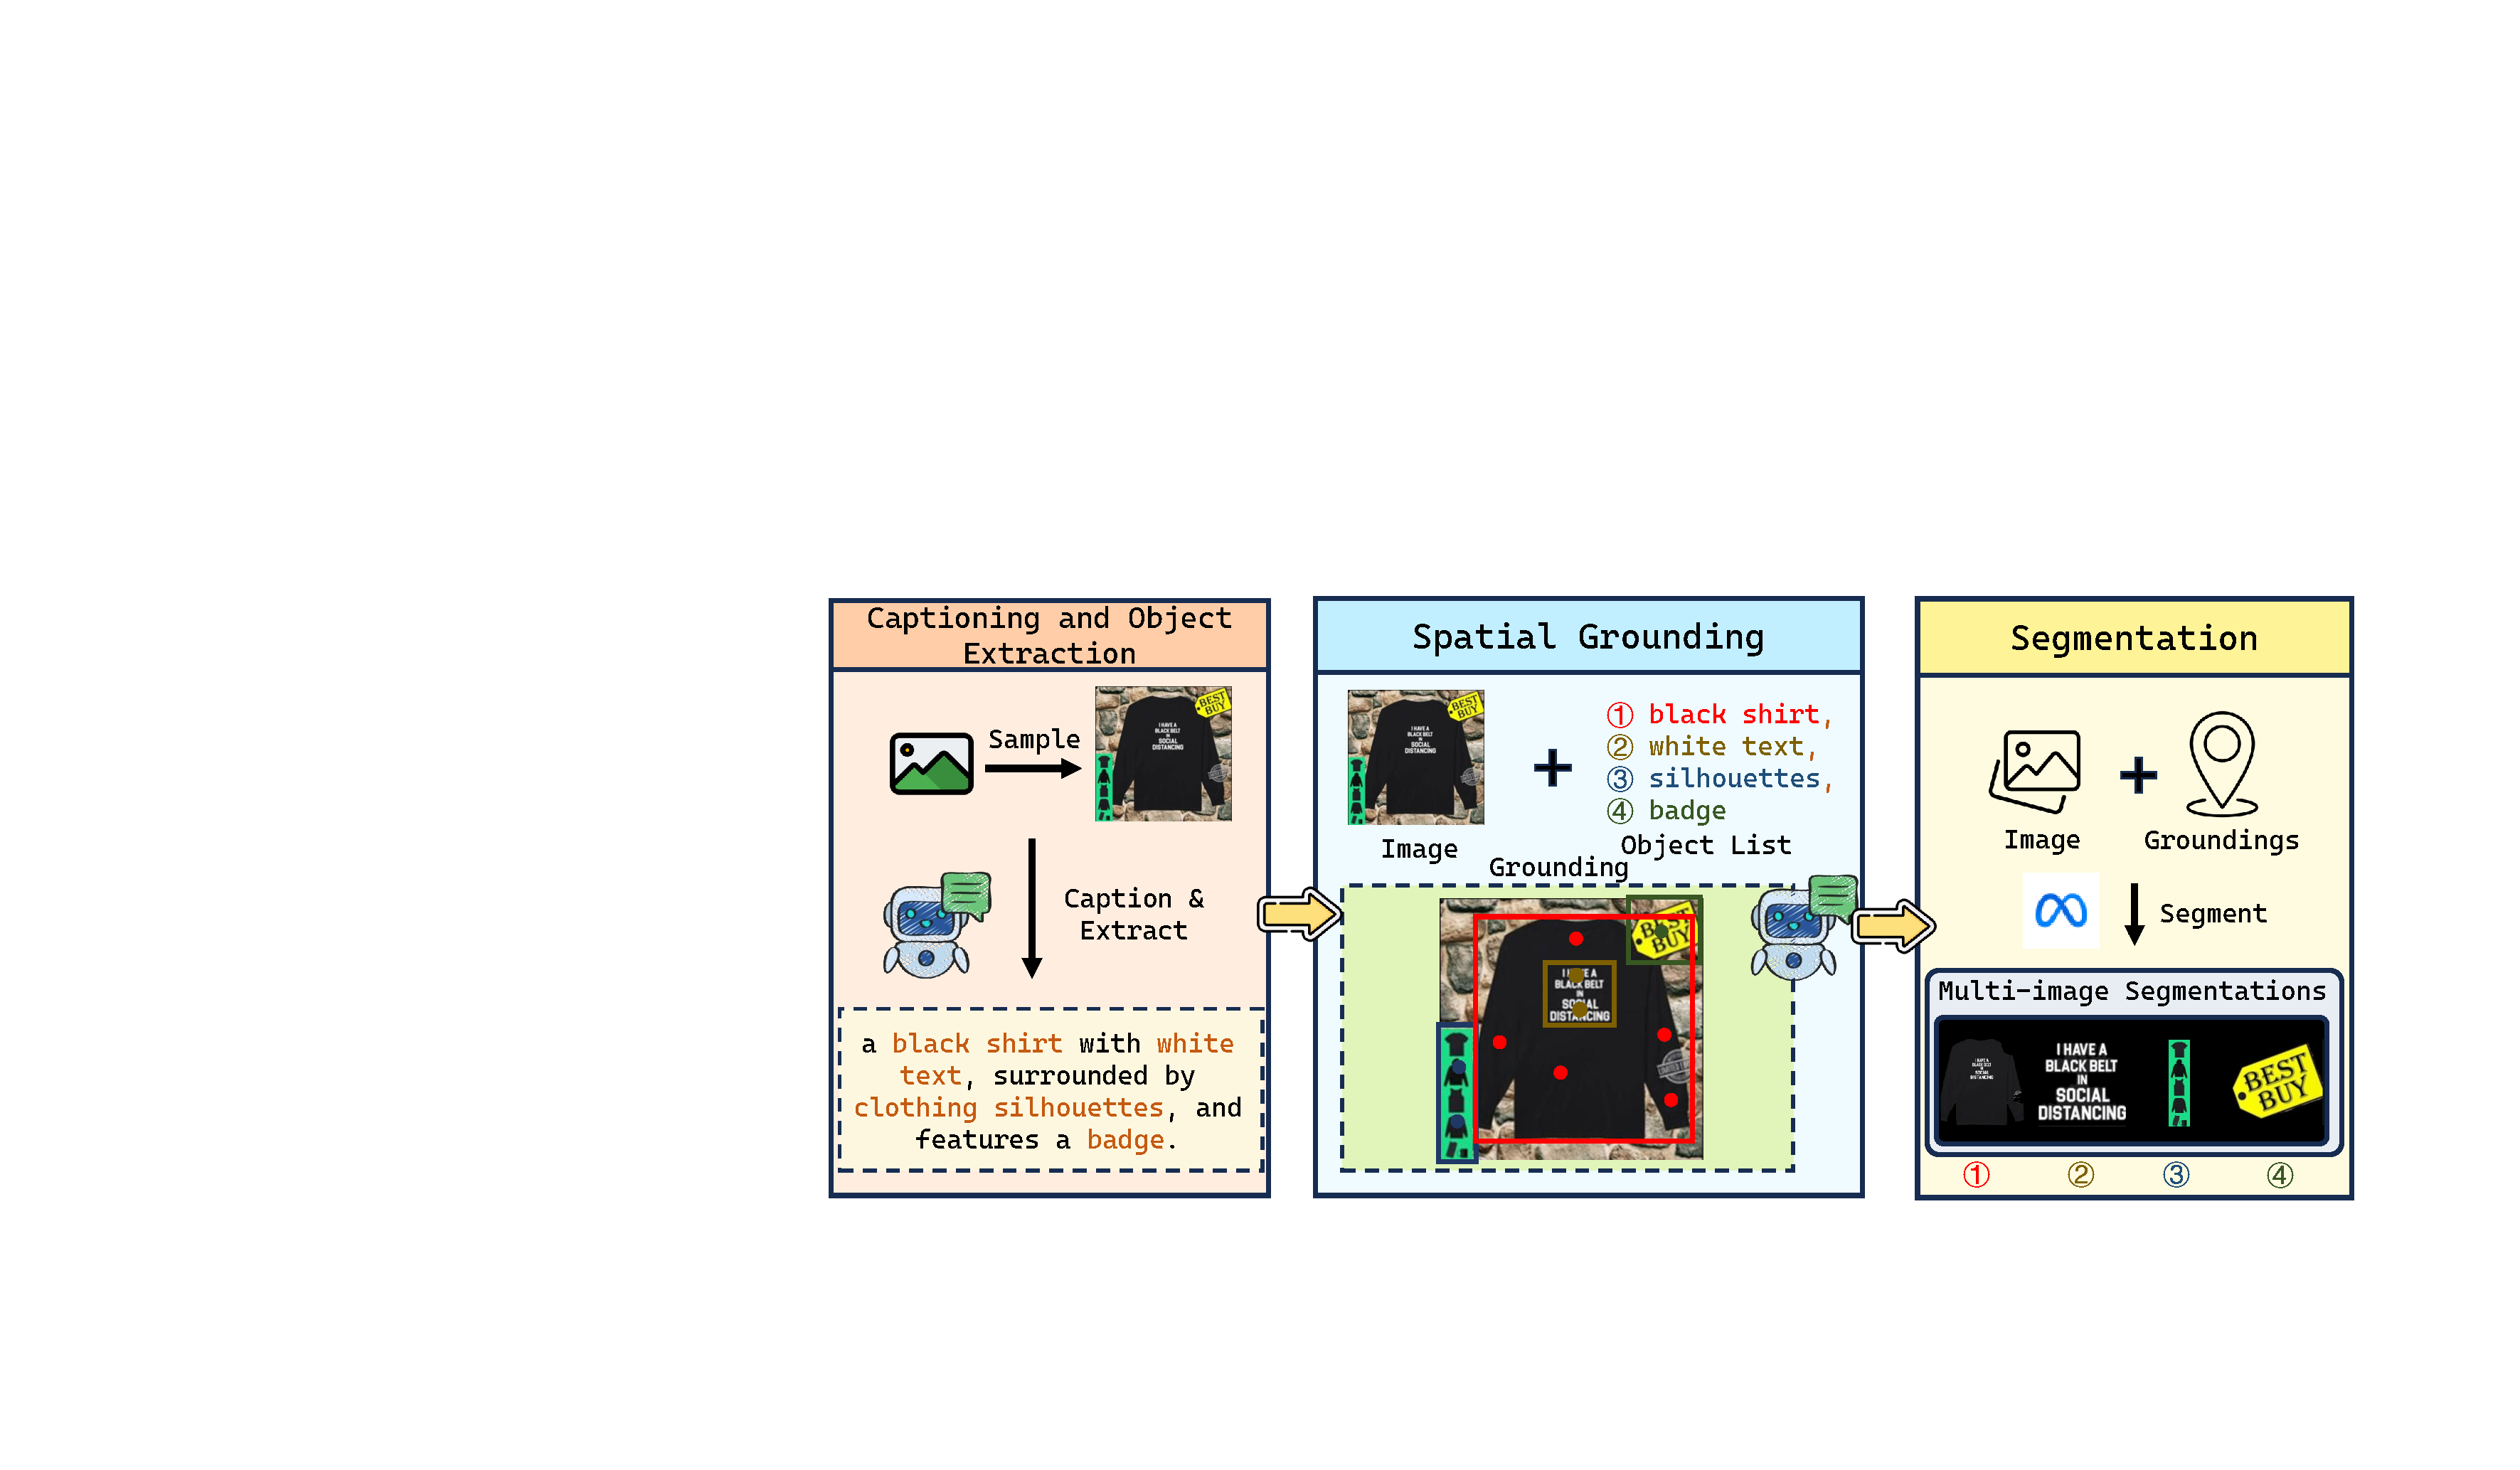
\includegraphics[width=1.0\textwidth]{figures/data_construct.pdf}
\caption{Illustration of the automatic data generation pipeline.}
\label{fig:construction}
\end{figure*}

\paragraph{Data Construction}
To support the large-scale training required for our two-stage paradigm, we developed an automated pipeline for generating high-quality multimodal training data, as shown in Figure~\ref{fig:construction}. This pipeline combines open-source image datasets with state-of-the-art vision-language models (VLMs) and segmentation models, enabling the construction of richly annotated image-text pairs with multiple segmented foreground objects without manual labeling:

\begin{itemize}[left=2pt]
\item \textbf{Captioning and Object Extraction:} A VLM is queried to generate a comprehensive caption describing prominent elements in the image, followed by extracting a list of concrete, distinct, and segmentable objects. This ensures that the generated data focus on tangible visual entities.
\item \textbf{Spatial Grounding:} For each extracted object, the VLM is queried again to identify its spatial location within the image, returning both a tight bounding box and several representative 2D keypoints. These spatial cues constrain the region of interest for subsequent segmentation, improving accuracy and reducing background noise.
\item \textbf{Segmentation:} A segmentation model is employed to extract object masks from the image, guided by the generated bounding boxes and keypoints. This step produces high-quality masks that are both semantically aligned with the object labels and spatially accurate.
\end{itemize}

By applying this automated process to a large corpus of open-source images, we construct a diverse multimodal dataset comprising captioned images annotated with multiple precisely segmented objects. This dataset forms a critical component of our training setup, particularly enabling the object segmentation and image recovery tasks in our training paradigm.


\section{Experiment Details}
\label{sec:Experiment_Details}

\subsection{Benchmark Details}
\label{sec:Benchmark_Details}

\paragraph{DreamBench++}
\label{app:DreamBench_Plus}

\textbf{Data Organization.}
DreamBench++~\citep{peng2025dreambenchpp} comprises 150 high-quality reference images, sourced from Unsplash, Rawpixel, and Google Images, encompassing a balanced mix of subjects. These are evenly divided into three broad categories: \textit{objects}, \textit{living subjects} (humans and animals), and \textit{styles} (illustrative, painterly, etc.), ensuring visual and conceptual diversity.

In total, DreamBench++ offers \textbf{1,350 prompts} ($150 \times 9$), representing a substantial scale-up over the original DreamBench (30 subjects $\times$ 25 prompts). Relative to DreamBench, the dataset is \textbf{5$\times$ larger in subjects} and \textbf{54$\times$ larger in prompts}, enabling broader evaluation of generative performance.

\textbf{Evaluation Metric.}
DreamBench++ adopts an automatic, GPT-4o-based evaluation protocol designed to closely mirror human judgment. Each generated image is assessed against both its reference image and its corresponding prompt, using two complementary axes:

\begin{itemize}[left=2pt, itemsep=0.5pt,topsep=0.5pt]
\item \textbf{Concept Preservation (CP):} Measures fidelity between the generated image and the reference. Key attributes include shape, color, texture, and facial details.
\item \textbf{Prompt Following (PF):} Evaluates how well the generation aligns with the prompt in terms of relevance, accuracy, completeness, and contextual appropriateness.
\end{itemize}

Each axis is scored on a \textbf{five-level ordinal scale} from 0 (Very Poor) to 4 (Excellent), avoiding the complexity and bias of pairwise comparisons.

\paragraph{DreamBench}
The original DreamBench~\citep{ruiz2023dreamboothfinetuningtexttoimage} dataset consists of 30 subjects, each paired with 25 prompts, totaling 750 prompt-image pairs. It serves as a foundational benchmark for evaluating personalized image generation models, focusing on the model's ability to maintain subject identity across diverse prompts.


\subsection{Baselines}
\label{sec:Baselines_Details}

We compare our method against various baselines, categorized as follows:

\begin{itemize}[left=2pt, itemsep=0.5pt,topsep=0.5pt]
\item \textbf{Textual Inversion}~\citep{gal2022imageworthwordpersonalizing} learns a new word embedding to represent a specific concept, enabling personalized image generation by incorporating the new token into prompts. It requires a few images of the subject and fine-tunes the embedding without altering the base model weights.
\item \textbf{DreamBooth}~\citep{ruiz2023dreamboothfinetuningtexttoimage}: DreamBooth fine-tunes a pre-trained text-to-image model to bind a unique identifier with the subject's visual concept, allowing for personalized generation. It requires several images of subject and modifies model weights to capture subject-specific details.

\item \textbf{BLIP-Diffusion}~\citep{li2023blipdiffusionpretrainedsubjectrepresentation}: This approach introduces a pre-trained multimodal encoder to provide subject representations for the diffusion generator, enabling controllable multimodal image generation. 

\item \textbf{KOSMOS-G}~\citep{Kosmos-G}: KOSMOS-G is a multimodal large language model designed for zero-shot image generation from interleaved vision-language inputs, including multiple images and text. It aligns the output space of a transformer-based causal language model with a diffusion-based image decoder using a lightweight AlignerNet and compositional instruction tuning. This architecture enables KOSMOS-G to perceive complex multimodal prompts and generate coherent, subject-driven images without modifying the base image decoder.

\item \textbf{Emu2}~\citep{emu2}: Emu2 is a 37-billion-parameter generative multimodal model trained on large-scale multimodal sequences with a unified autoregressive objective. It exhibits strong in-context learning abilities for various multimodal tasks, including visual prompting and object-grounded generation.

\item \textbf{IP-Adapter}~\citep{ye2023ip-adapter}: IP-Adapter is a lightweight adapter that enables image prompt capability for pre-trained text-to-image diffusion models. It integrates image features into the generation process without modifying the base model, supporting flexible and efficient image-to-image generation.

\item \textbf{DreamEngine}~\citep{dreamengine}: DreamEngine is a unified framework that integrates multimodal encoders with diffusion models through a two-stage training approach, enabling advanced text-image interleaved control and achieving state-of-the-art performance in generating images with complex, concept-merged inputs.

\item \textbf{Unified-IO 2}~\citep{lu2023unifiedio2}: Unified-IO 2 is an autoregressive multimodal model capable of understanding and generating images, text, audio, and actions. It tokenizes various modalities into a shared semantic space and processes them with a single encoder-decoder transformer. Trained from scratch on a large multimodal pre-training corpus and fine-tuned on an ensemble of 120 datasets, Unified-IO 2 achieves state-of-the-art performance on the GRIT benchmark and strong results across more than 35 benchmarks. 

\item \textbf{Lumina-mGPT}~\citep{2024lumina}: Lumina-mGPT is a multimodal autoregressive models designed for flexible photorealistic text-to-image generation. It employs a pretrained decoder-only transformer as a unified framework for modeling multimodal token sequences. Through multimodal Generative PreTraining (mGPT) and subsequent Flexible Progressive Supervised Finetuning (FP-SFT) and Omnipotent Supervised Finetuning (Omni-SFT), Lumina-mGPT demonstrates versatile multimodal capabilities, including visual generation tasks, controllable generation tasks and vision-language tasks. 

\end{itemize}



\section{Qualitative Study}
\label{sec:Qualitative_Study}

\subsection{Image Reconstruction}
\label{sec:Reconstruction}

\begin{figure*}[t]
\centering
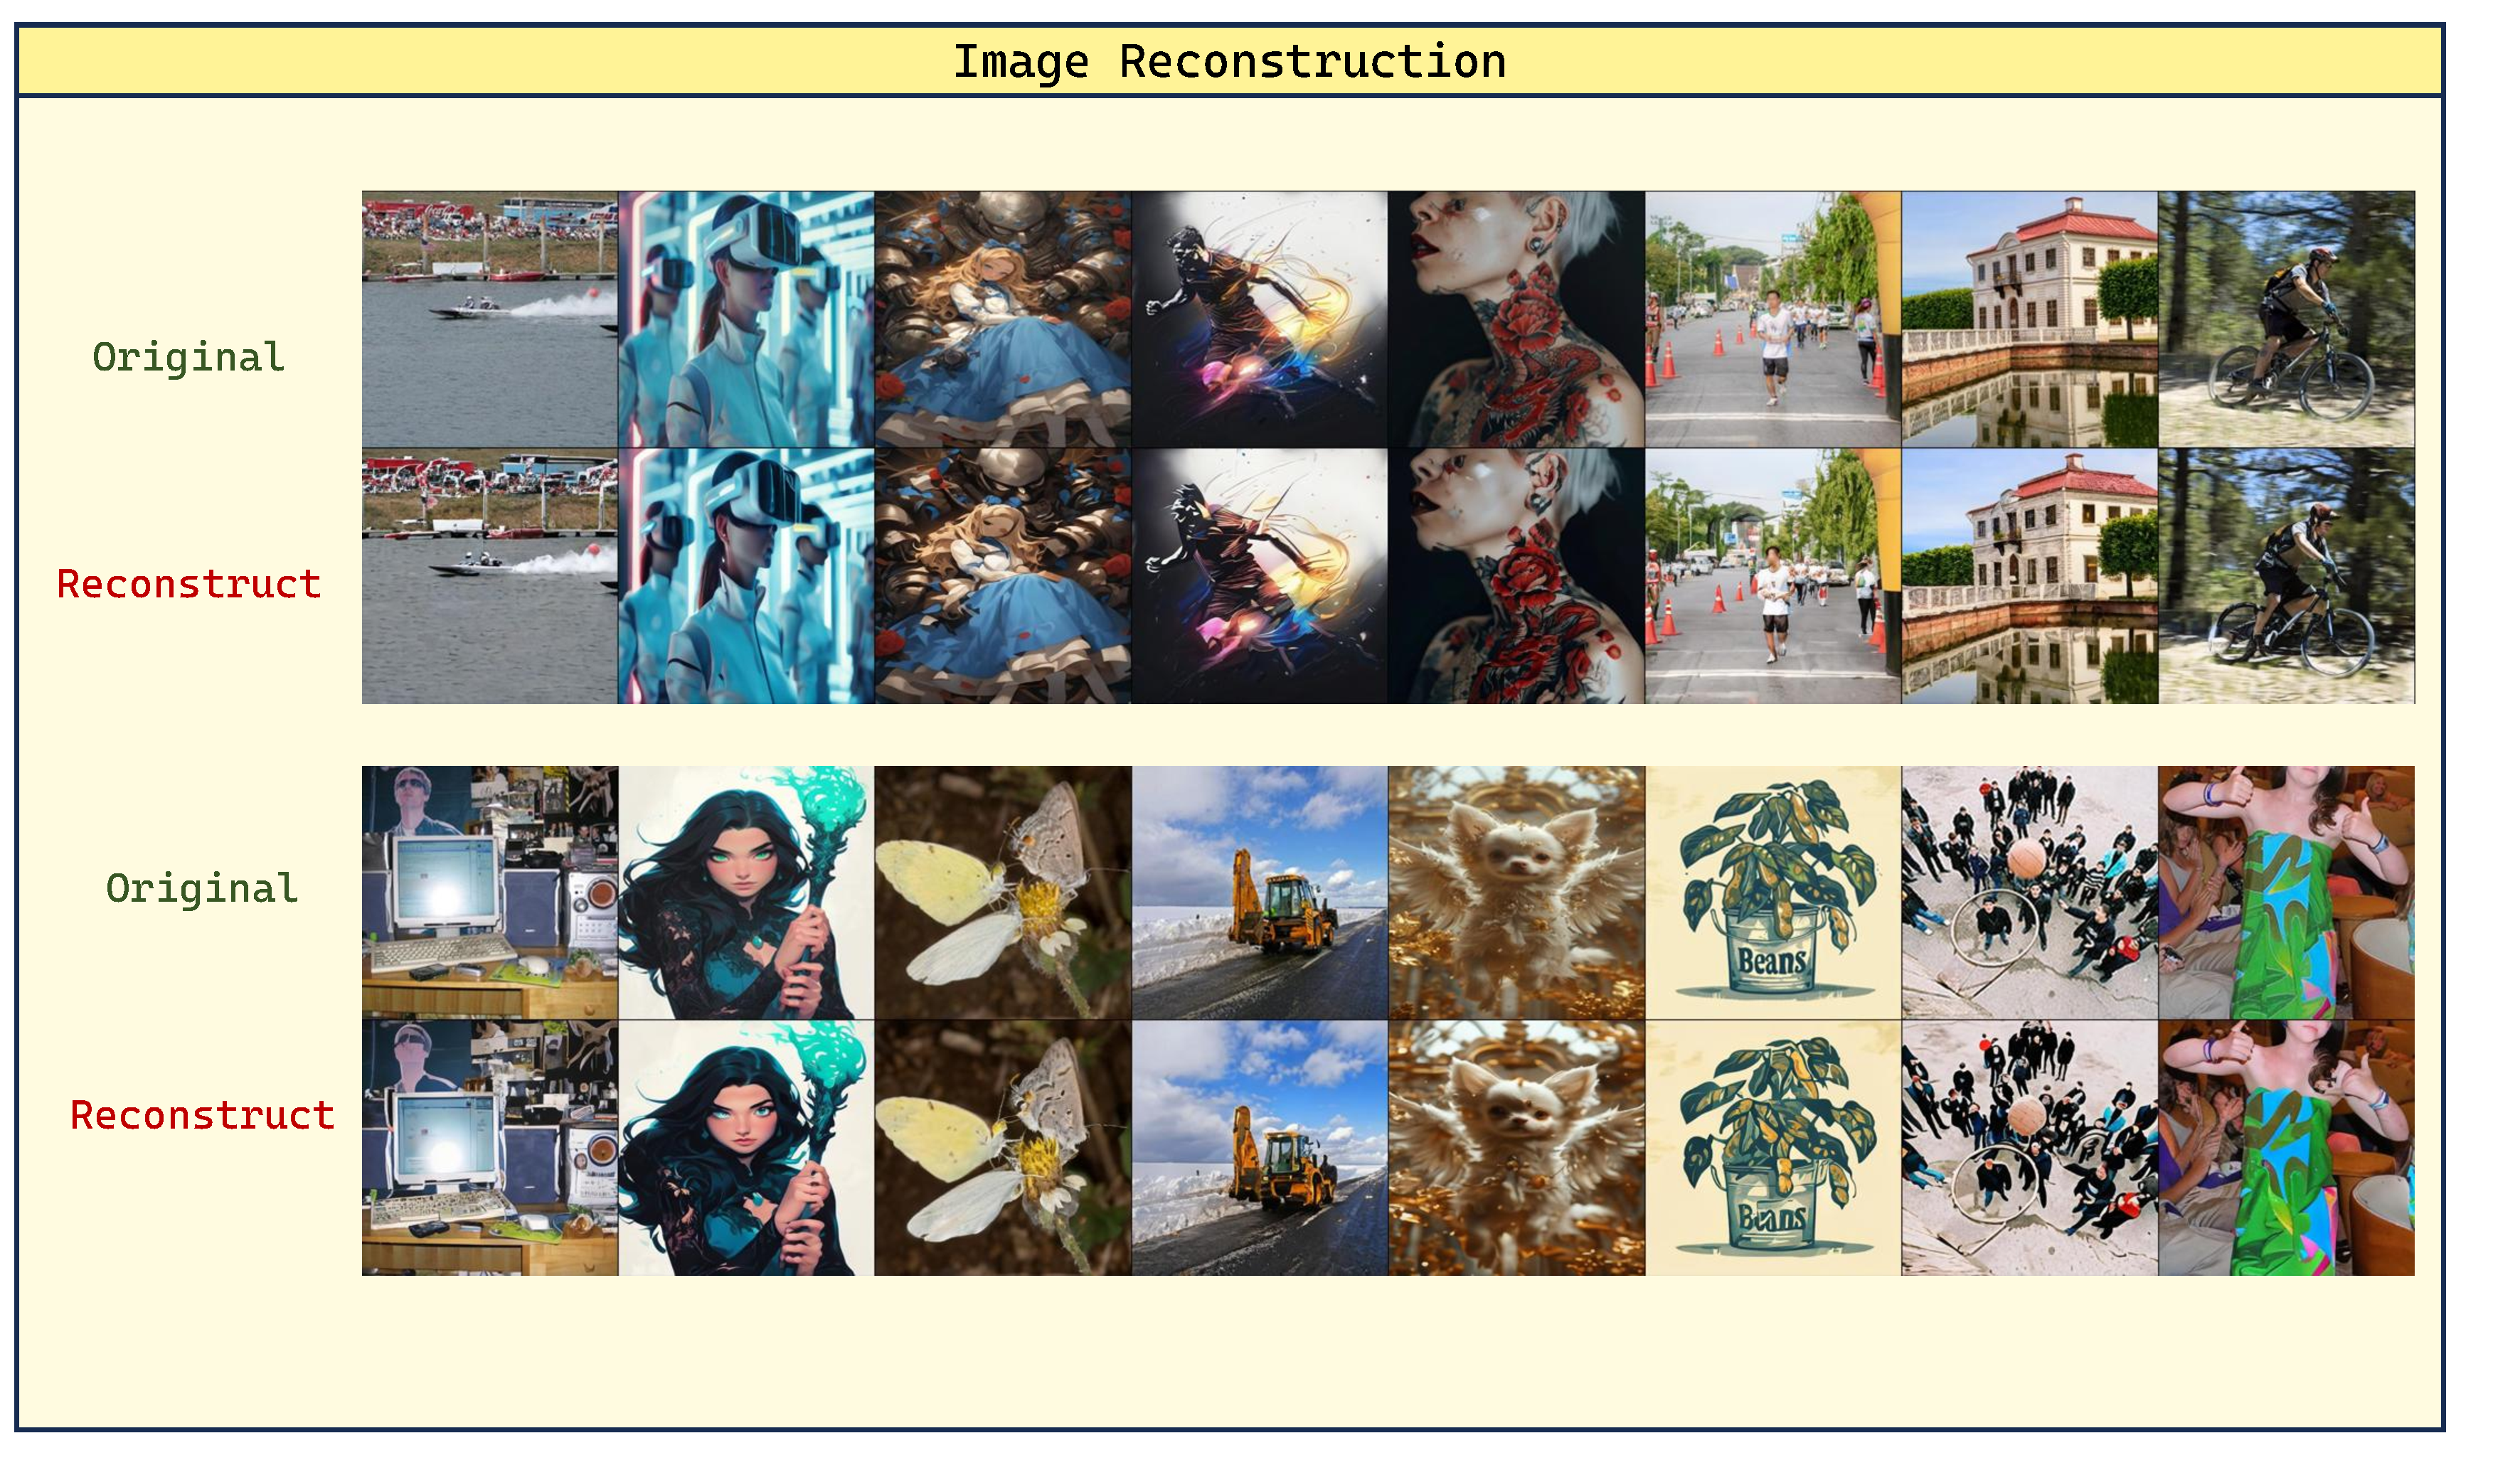
\includegraphics[width=0.85\textwidth]{figures/reconstrucion.pdf}
\caption{Qualitative comparison of image reconstruction results using \model.}
\label{fig:reconstruction}
\end{figure*}

\begin{figure*}[t]
\centering
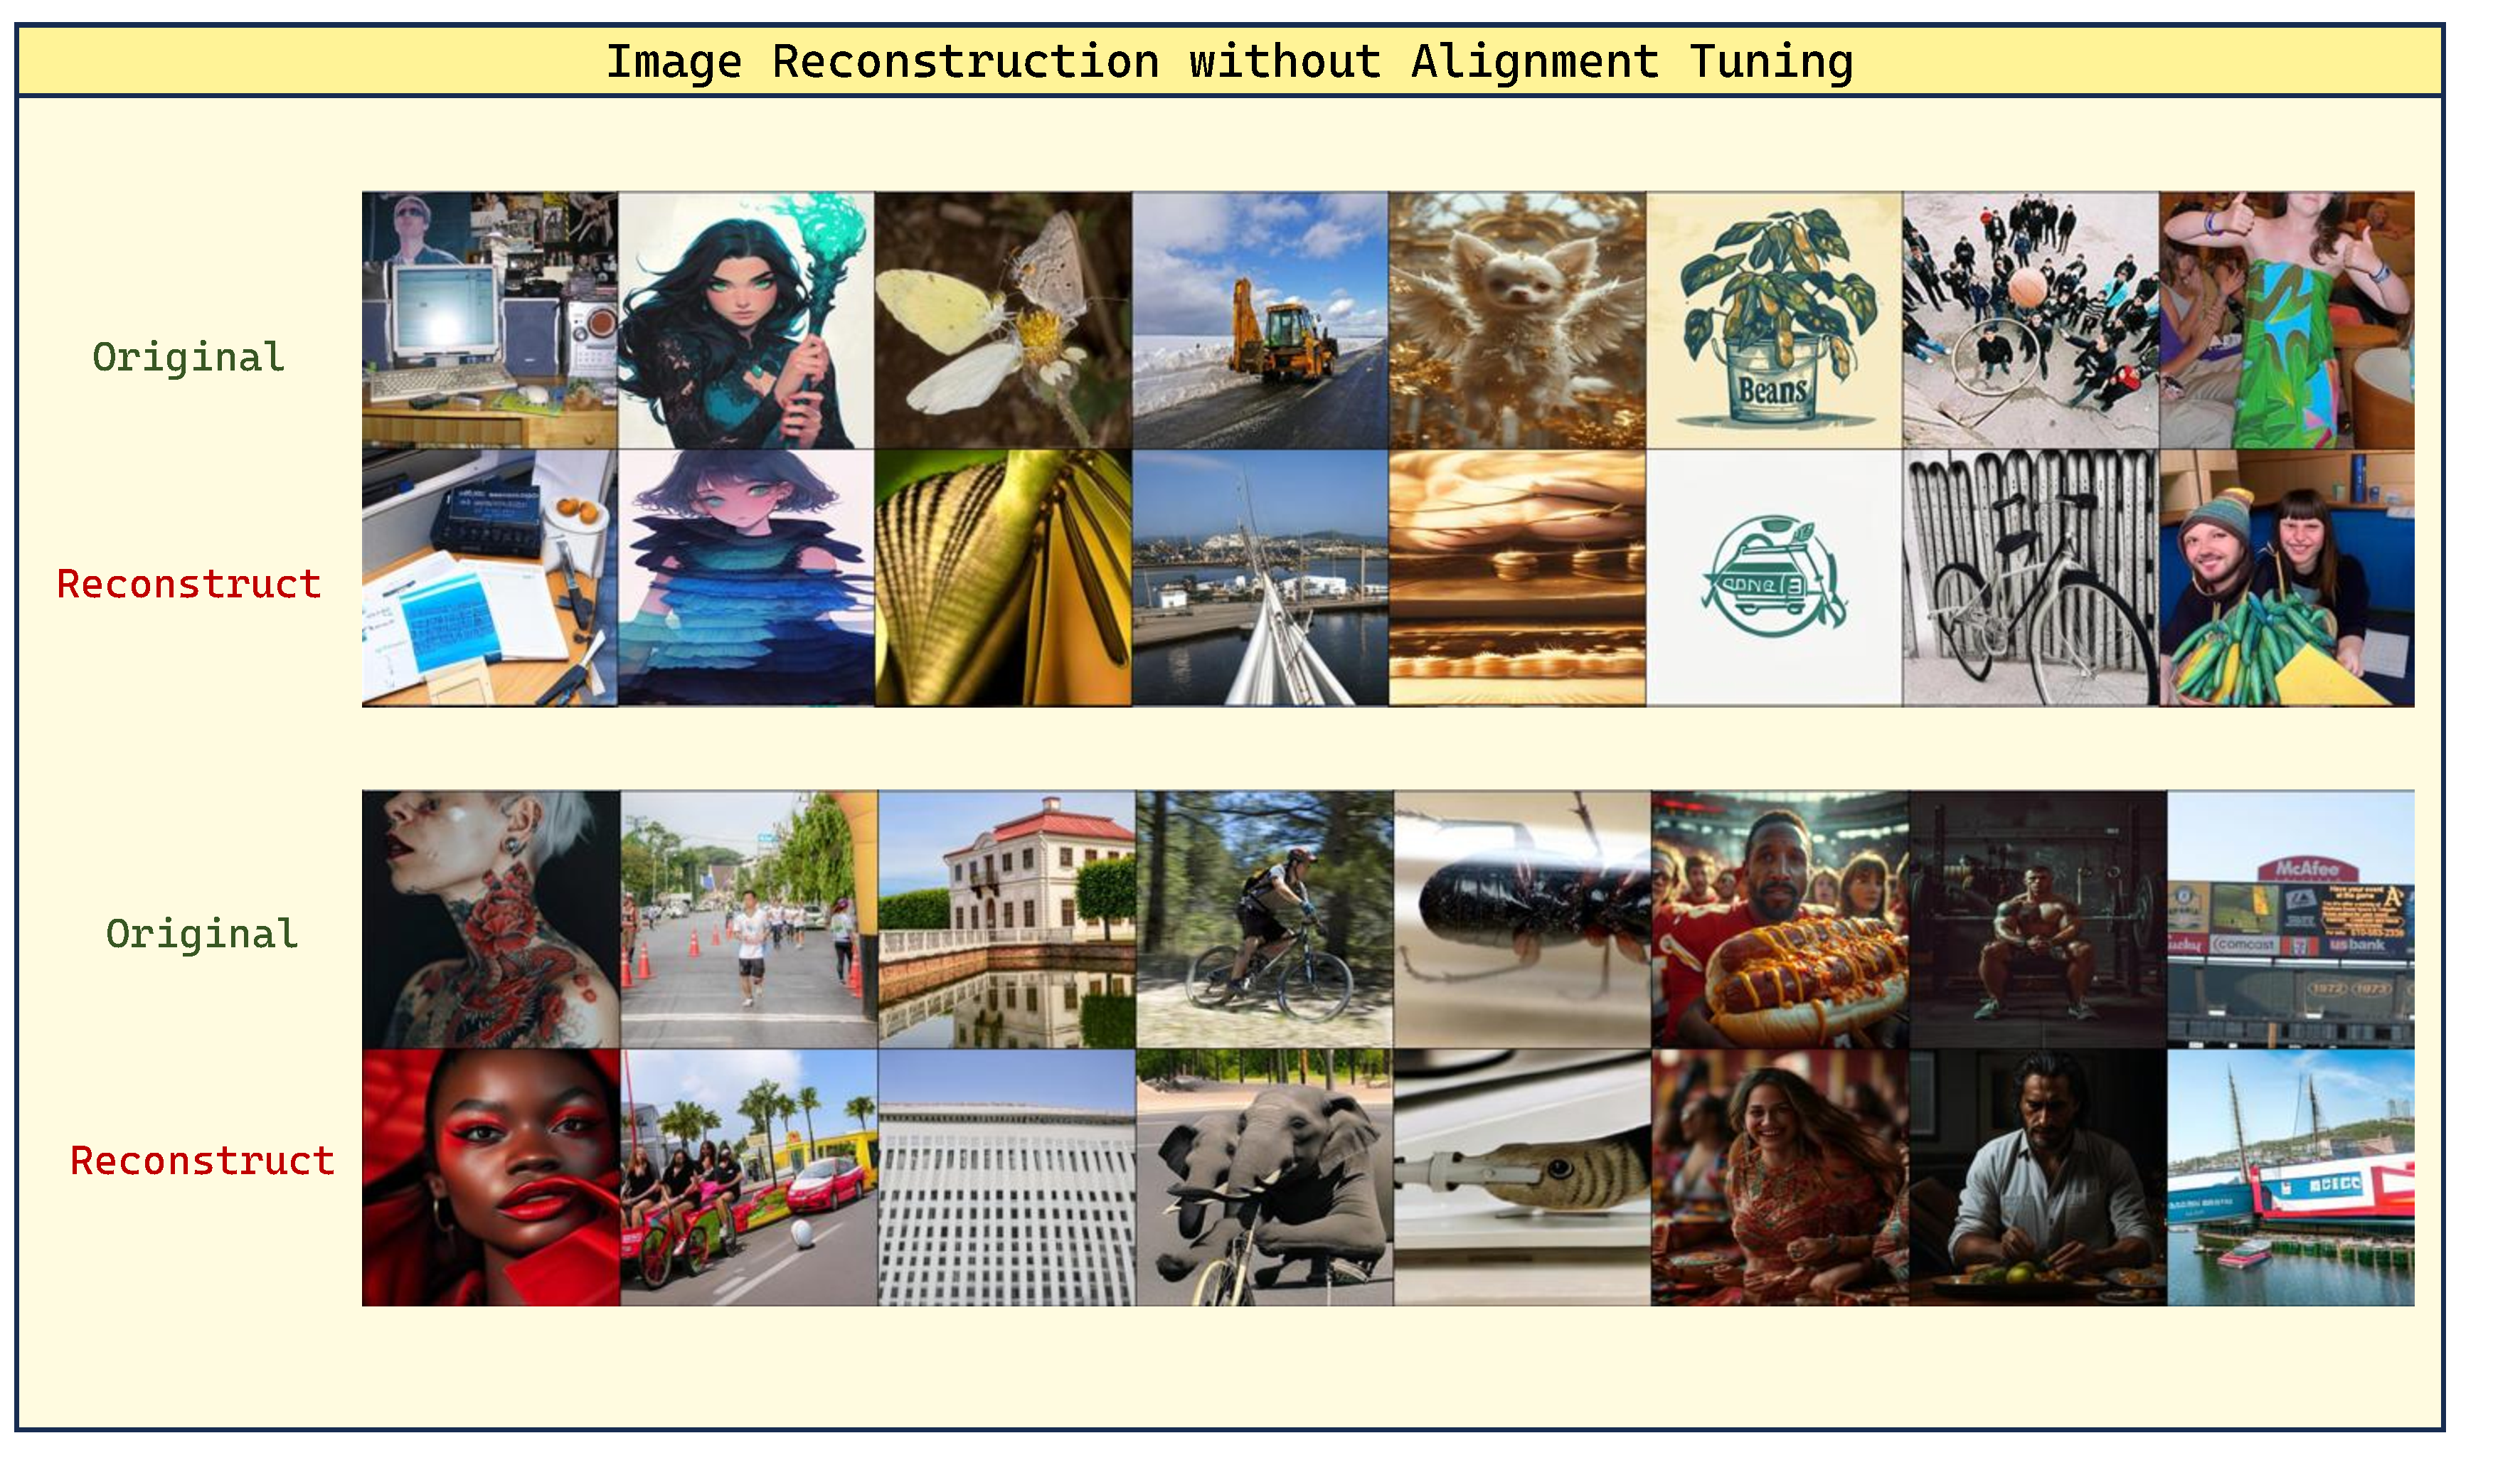
\includegraphics[width=0.85\textwidth]{figures/reconstrucion_wo_alignment.pdf}
\caption{Image reconstruction results of \model \textit{without} alignment tuning.}
\label{fig:reconstruction_wo_align}
\end{figure*}

As illustrated in Figures~\ref{fig:reconstruction} and \ref{fig:reconstruction_wo_align}, \model demonstrates strong image reconstruction capabilities following two-stage training. Notably, it is able to effectively reconstruct input images and preserve fine-grained visual details, even when input images are of low resolution (224×224) and outputs are generated at 512×512 resolution.

In contrast, when alignment tuning is omitted, although the model benefits from the pretrained multimodal encoder and the proposed architecture, it tends to treat the input image as a visual prompt akin to a caption. As shown in Figure~\ref{fig:reconstruction_wo_align}, this leads to outputs that resemble descriptive interpretations of the input rather than faithful reconstructions. Consequently, visual fidelity and spatial consistency degrade significantly without alignment tuning.

\subsection{Text-guided Image Segmentation}
\label{sec:Segmentation}


\begin{figure*}[t]
\centering
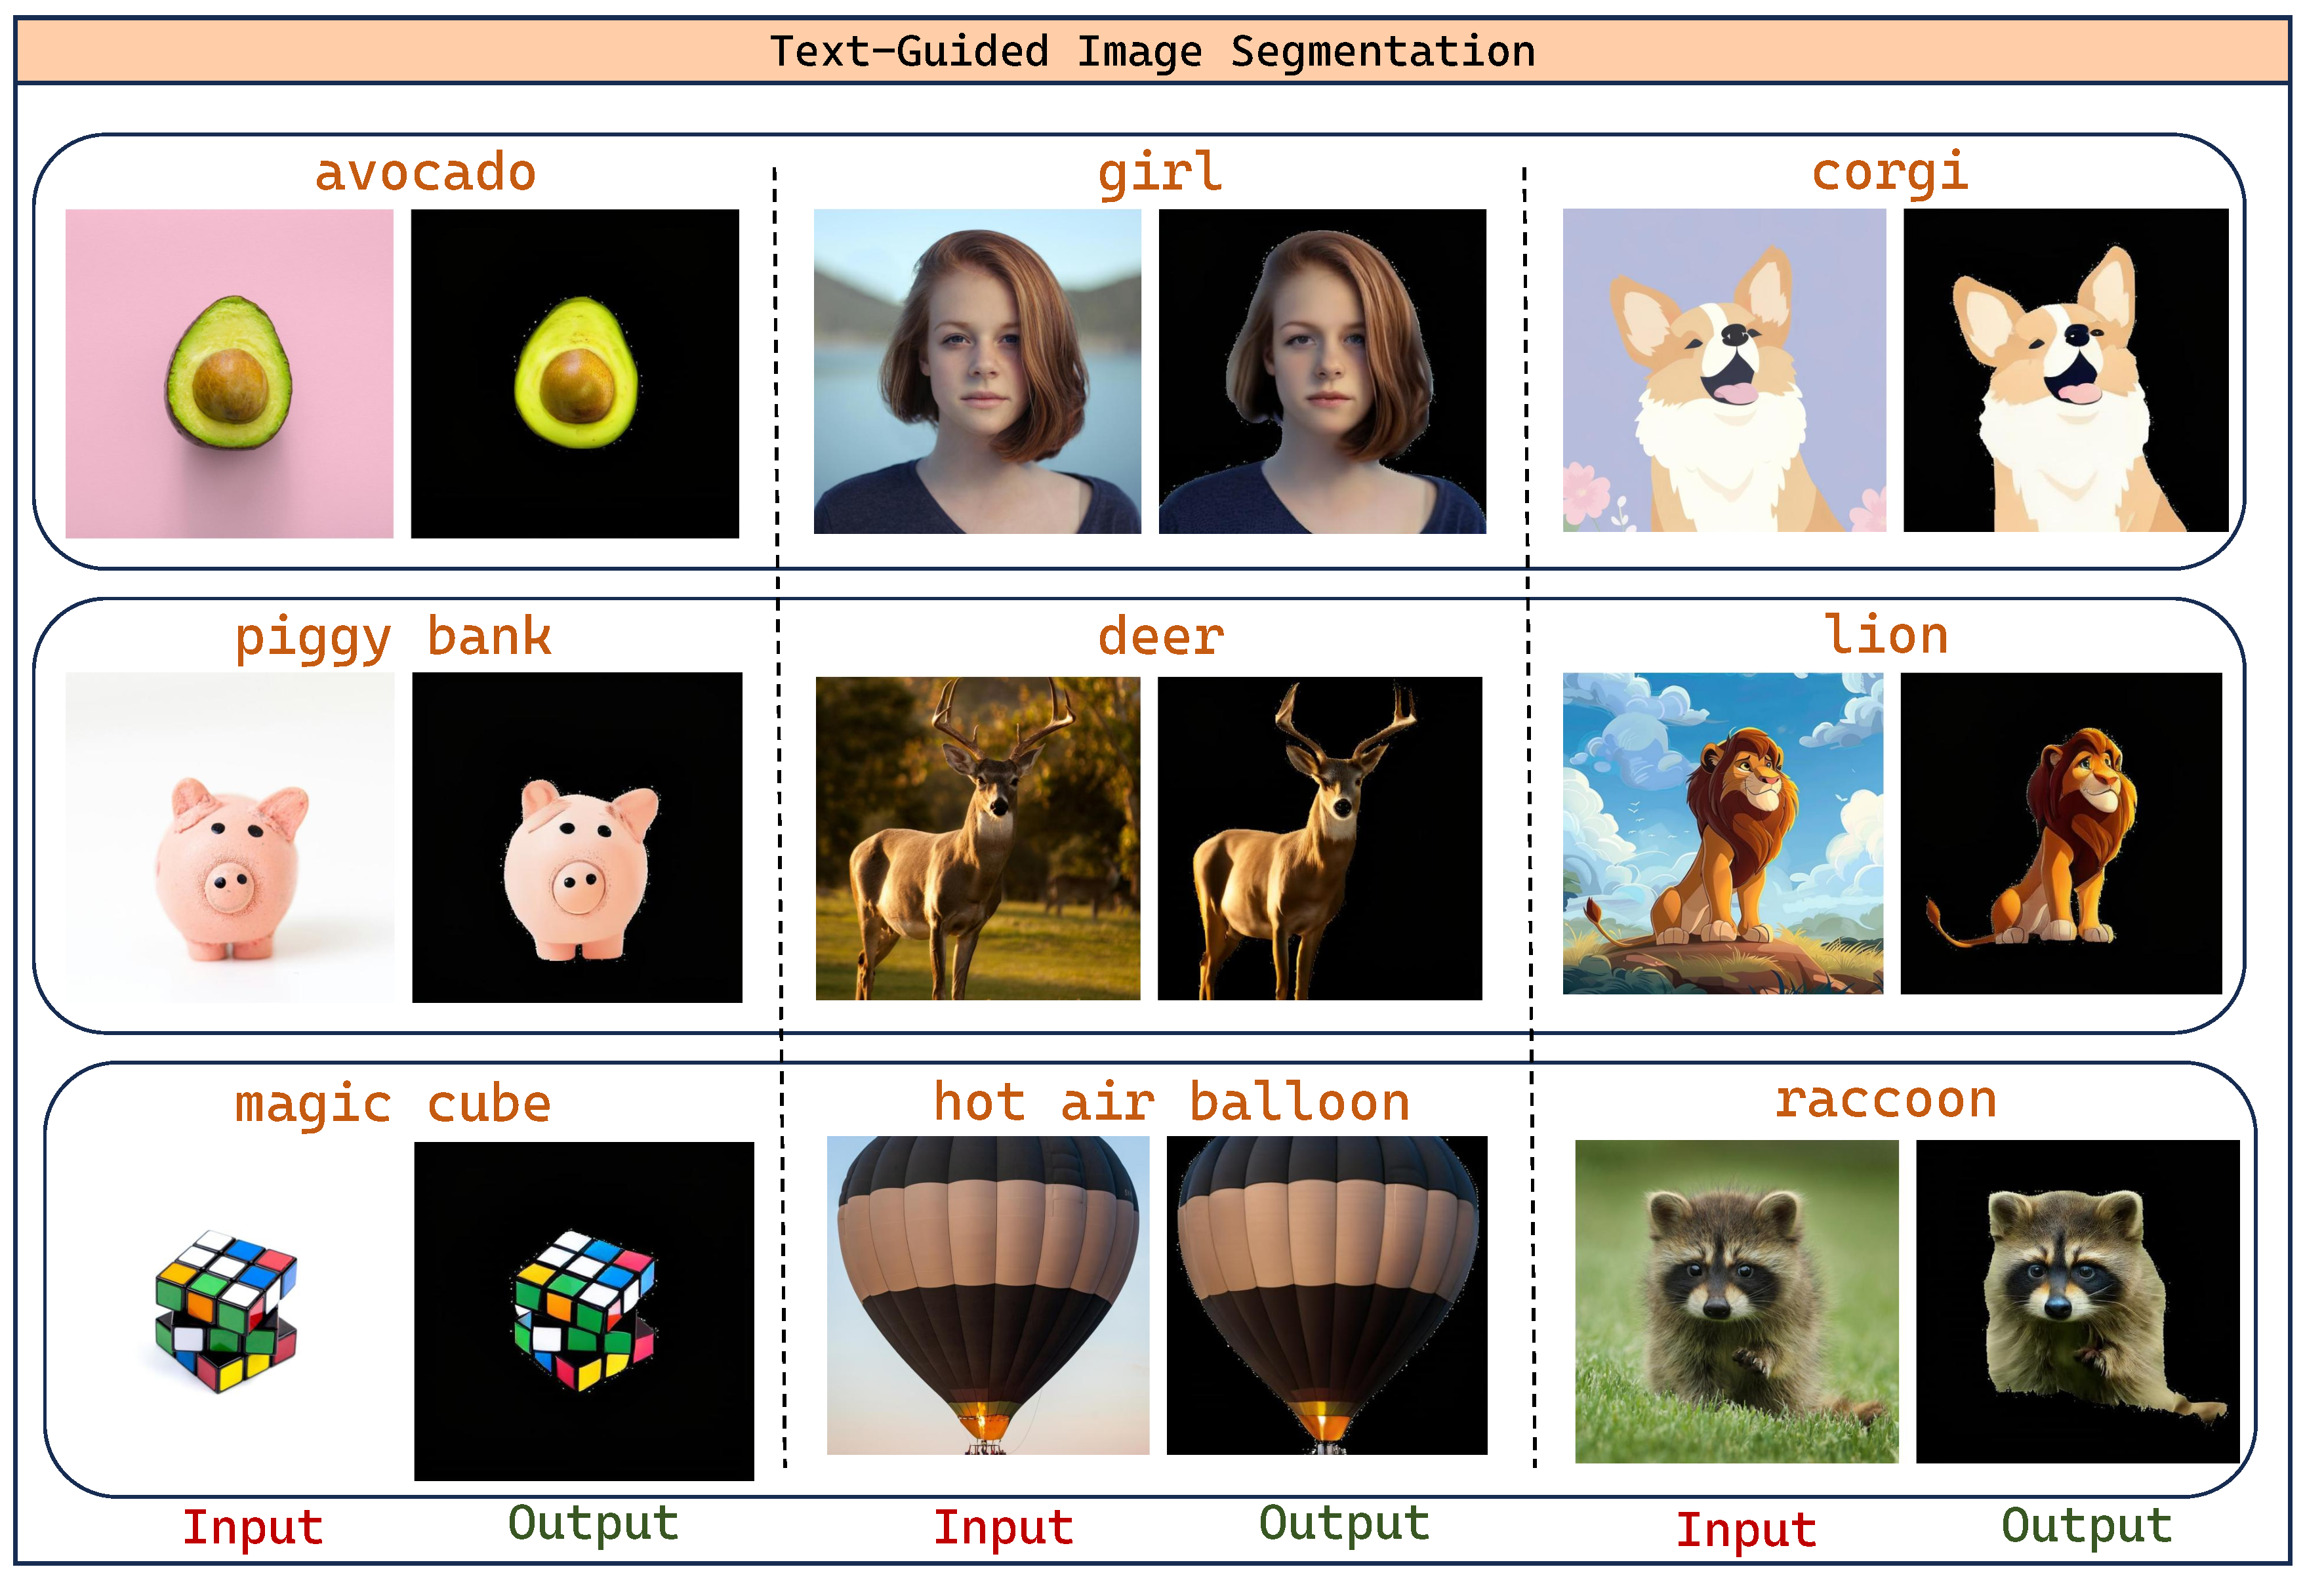
\includegraphics[width=1.0\textwidth]{figures/segmentation_example.pdf}
\caption{Qualitative results of text-guided image segmentation using \model.}
\label{fig:segmentation_example}
\end{figure*}

We evaluate \model on the DreamBench\texttt{++} benchmark to assess its performance in text-guided image segmentation. As demonstrated in Figure~\ref{fig:segmentation_example}, \model successfully identifies and segments visual concepts corresponding to the given textual prompts. These results highlight the model's ability to generalize across tasks and showcase its robust multimodal understanding and generation.

\subsection{Multi-Image Generation}
\label{sec:Multi-Image}

\begin{figure*}[t]
\centering
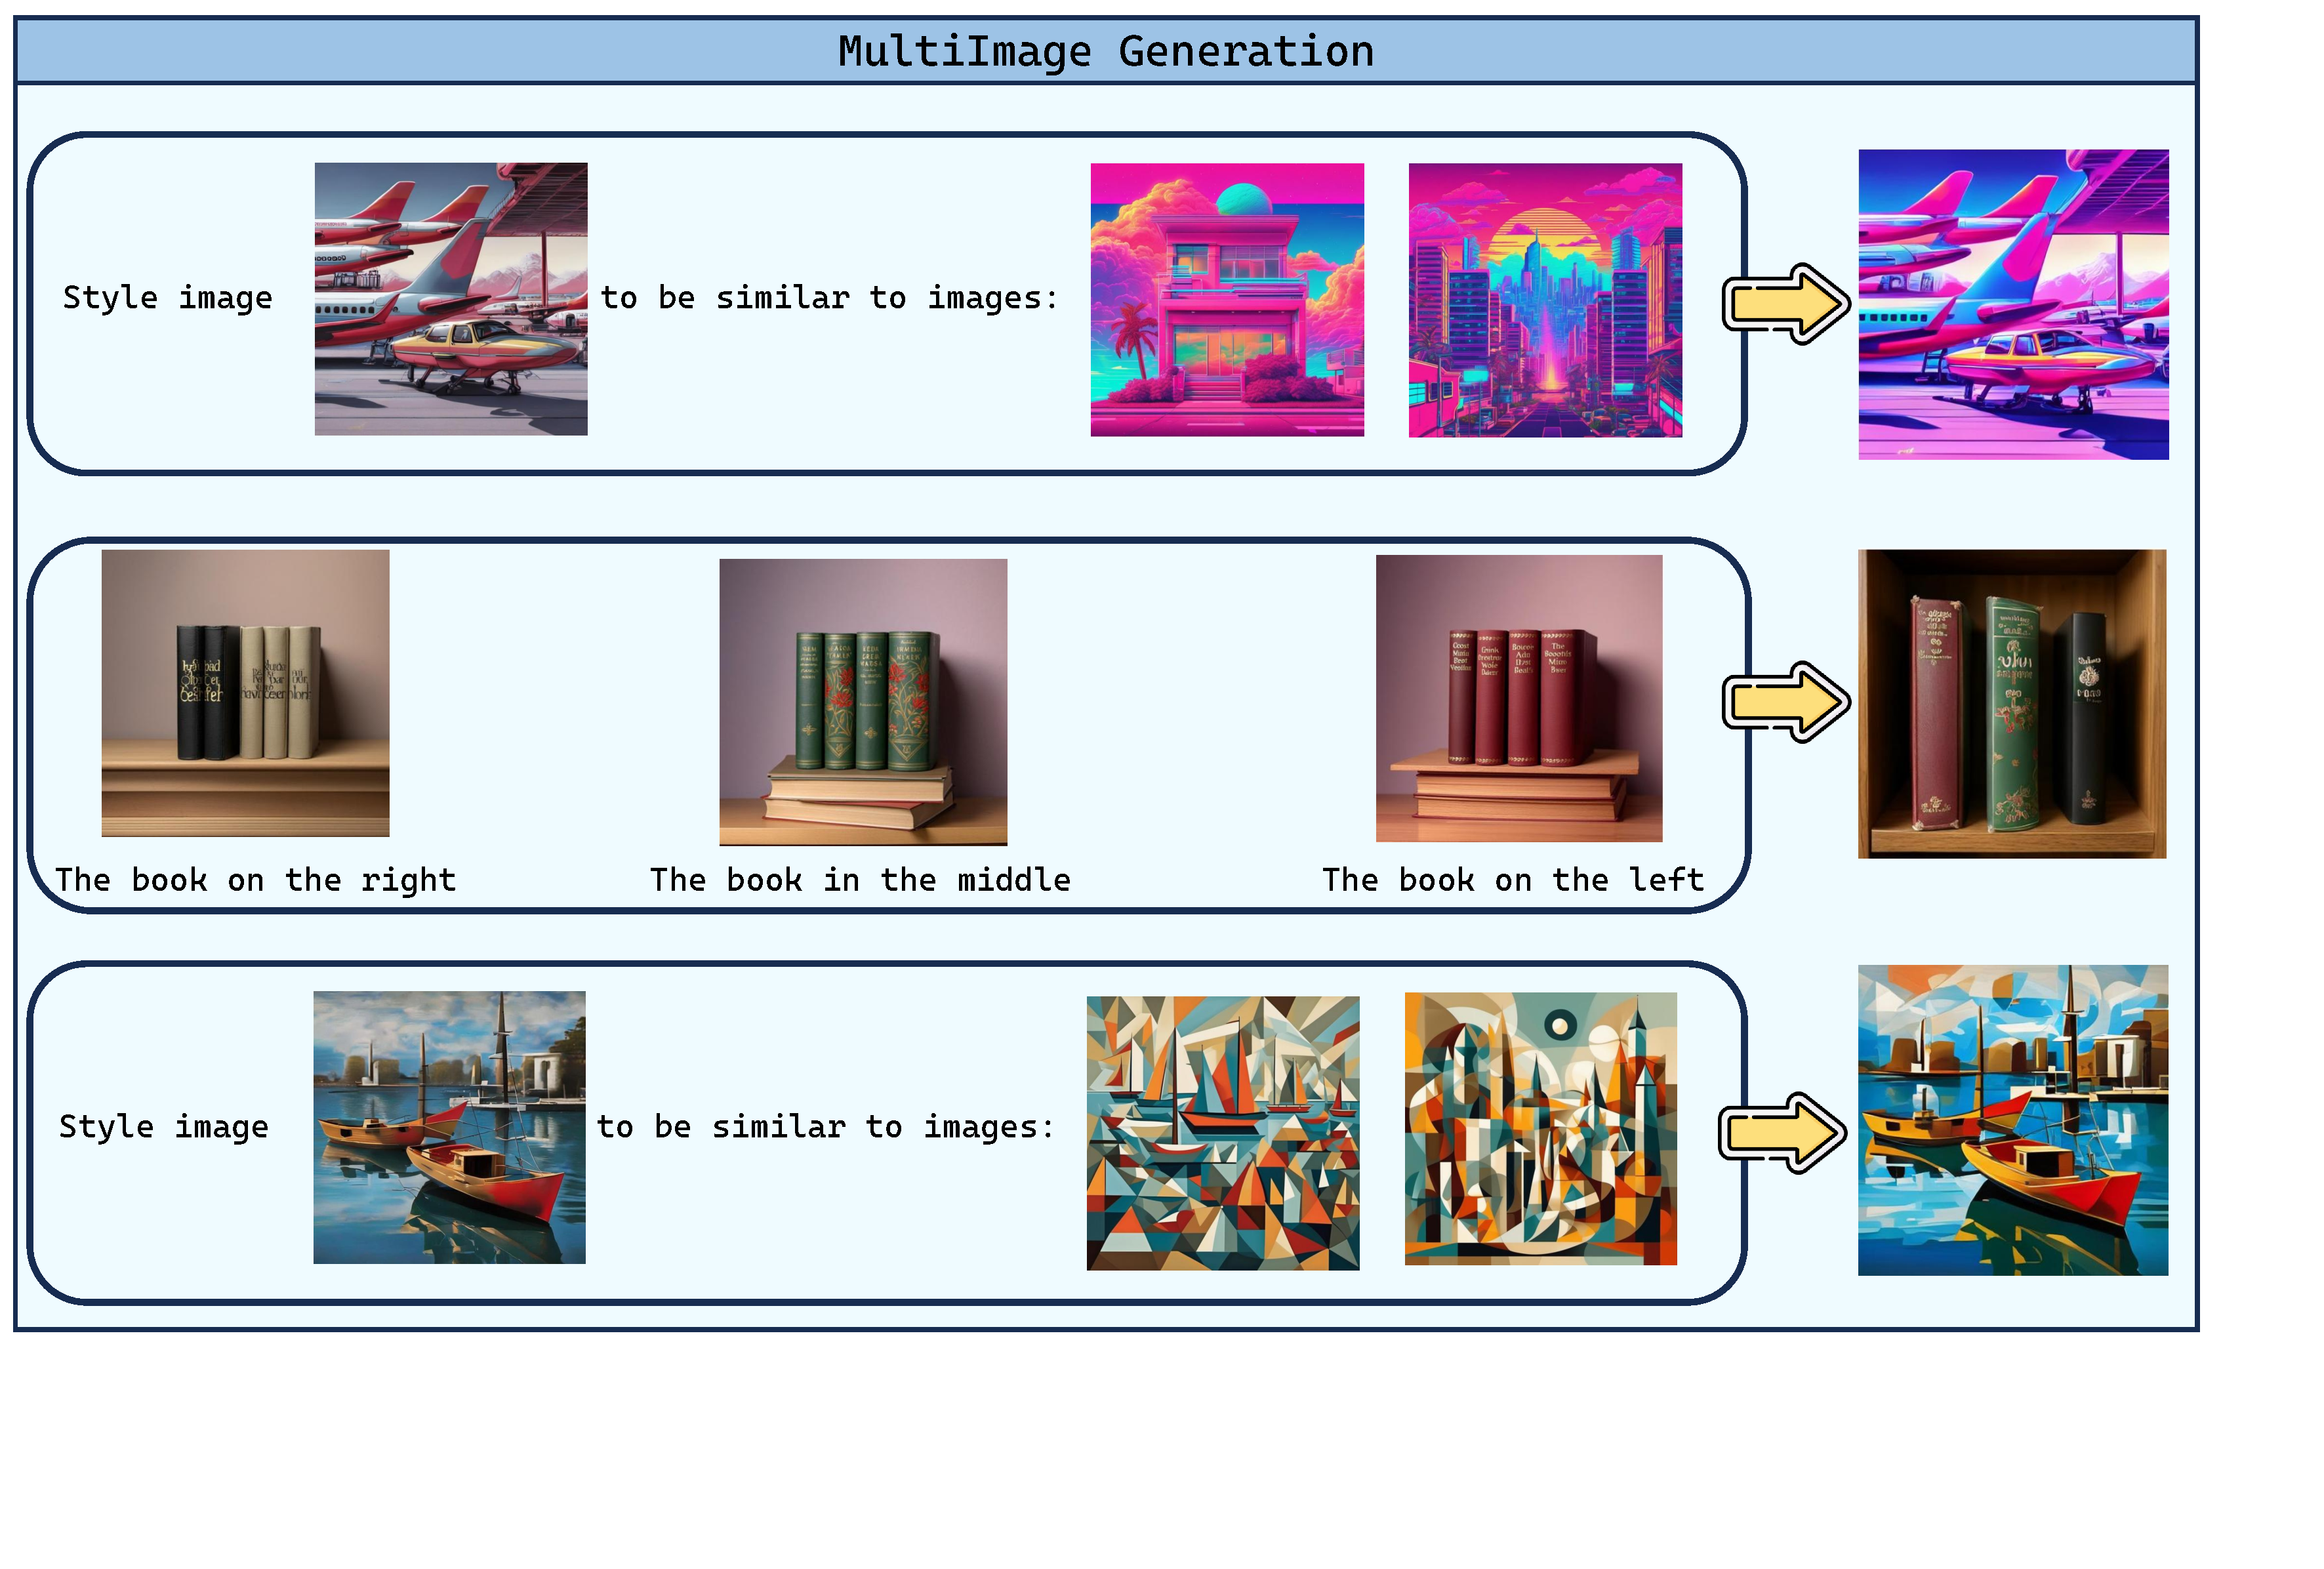
\includegraphics[width=0.85\textwidth]{figures/multi_img.pdf}
\caption{Qualitative results for multi-image generation.}
\label{fig:multi_image}
\end{figure*}

We evaluate \model on multi-image generation tasks using the X2I dataset~\citep{OmniGen}. As shown in Figure~\ref{fig:multi_image}, the model is capable of generating visually consistent outputs conditioned the multi-image inputs. The generated images reflect coherent semantics, style, and layout across the samples.

\subsection{Multimodal In-Context Image Generation}
\label{sec:mmicl}

\begin{figure*}[t]
\centering
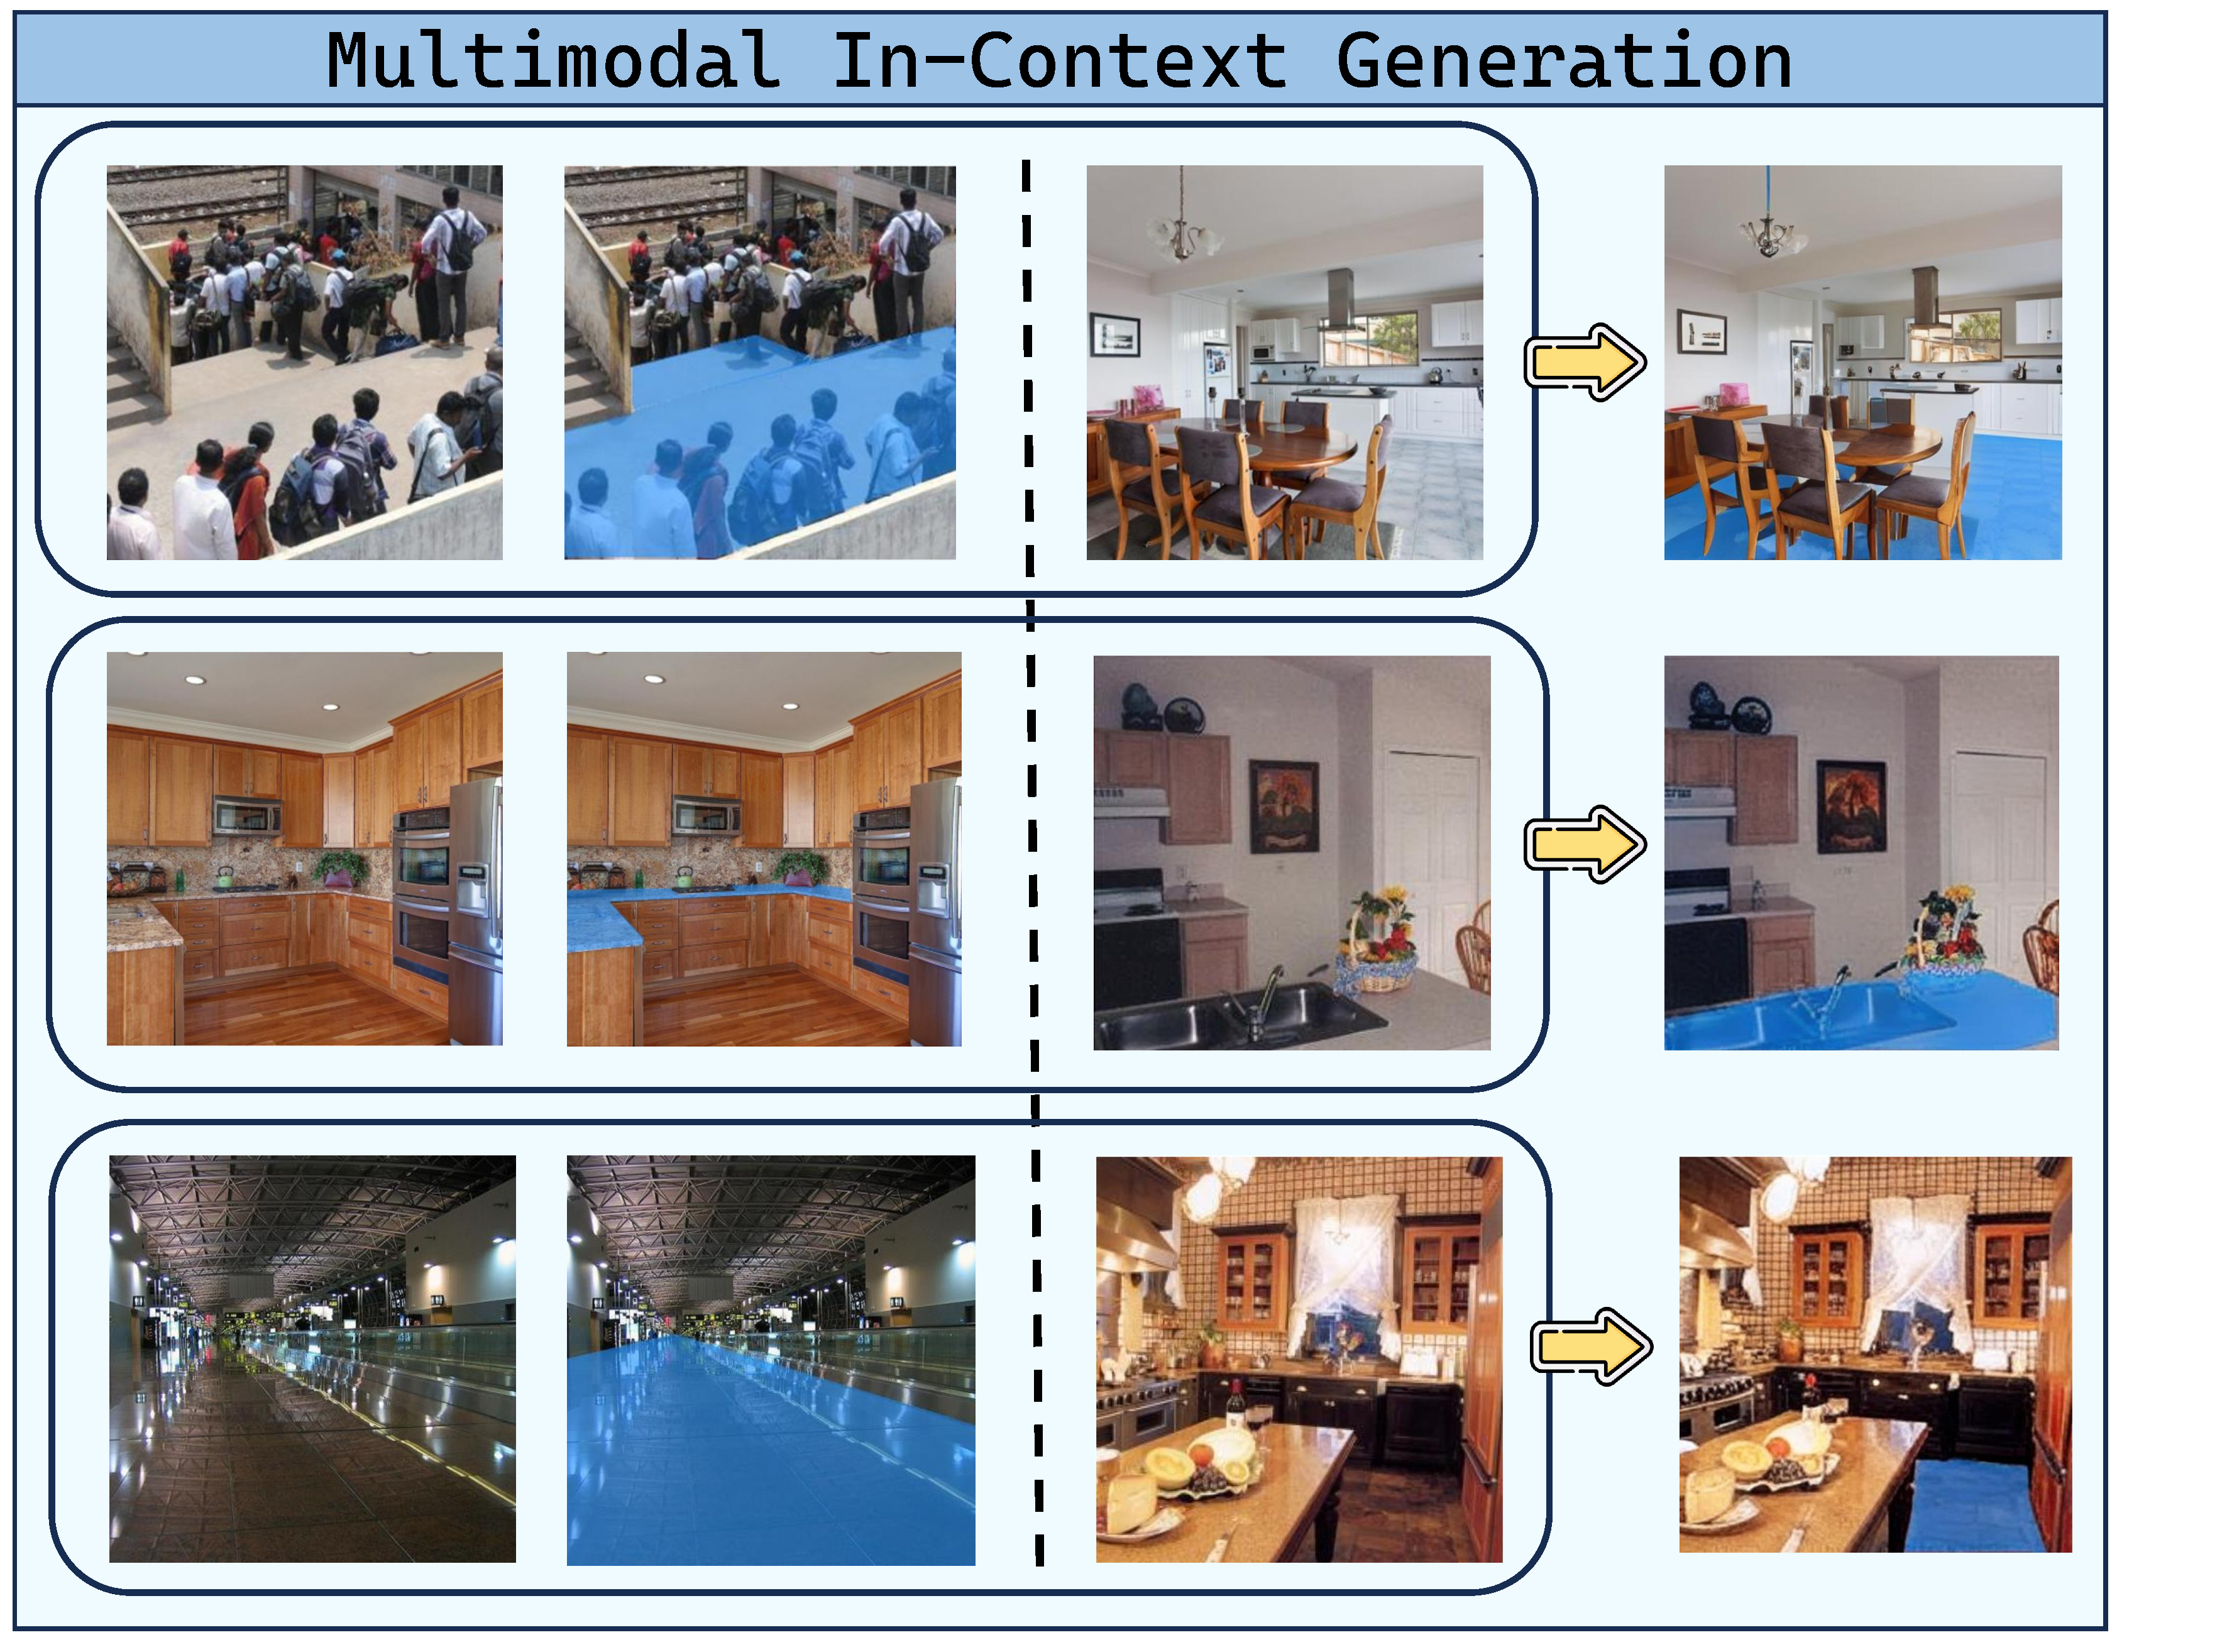
\includegraphics[width=0.75\textwidth]{figures/icl_exp.pdf}
\caption{Qualitative examples from multimodal in-context image generation. The model adapts to patterns in the visual context.}
\label{fig:icl_example}
\end{figure*}

To assess \model's few-shot generalization capabilities, we evaluate it on the multimodal in-context image generation task using the X2I-ICL dataset~\citep{OmniGen}. As illustrated in Figure~\ref{fig:icl_example}, \model learns to synthesize images that follow the stylistic patterns demonstrated in the in-context examples. This indicates its capability to infer complex visual trends and align generation with image context.

\section{Versatility Across Different Multimodal Tasks}
\label{app:applications}

To assess the broad applicability of our proposed framework, we evaluate \model across a diverse set of multimodal generation tasks, including text-guided image segmentation, subject-driven image generation, multi-image generation, and multimodal in-context learning. For each task, we apply supervised fine-tuning where necessary, ensuring robust generalization while maintaining architectural consistency.

\paragraph{Image Segmentation.}
We evaluate this task directly after Stage 1 training, without additional fine-tuning. The model demonstrates strong object localization and mask precision from prompt-aligned inputs, confirming the effectiveness of the proposed training pipeline and segmentation-aware data construction process.

\paragraph{Subject-driven Image Generation.}
This task is evaluated using the model at the end of Stage 2. No additional task-specific tuning is applied. The model successfully generates high-fidelity, identity-preserving images consistent with subject descriptors.

\paragraph{Multi-Image Generation.}
We fine-tune the Stage 2 model on a subset of X2I-subject-driven~\citep{OmniGen} dataset for two additional epochs using a reduced learning rate of $5 \times 10^{-5}$. All other optimization settings remain consistent with Stage 2. The dataset is split into disjoint training and test sets, and quantitative results are reported on the test split. The model learns to generate visually diverse yet semantically aligned images for the same input.

\paragraph{Multimodal In-Context Learning.}
We fine-tune the model for 10 epochs on the X2I-ICL dataset~\citep{OmniGen}, which features sequences of input-output pairs for in-context generalization. We use a learning rate of $5 \times 10^{-5}$ and ensure a strict train-test separation. The model adapts to context examples and generates new samples following the observed patterns, showing strong in-context learning performance without explicit prompting engineering.

\paragraph{Conclusion.}
The qualitative results presented in Section~\ref{sec:Qualitative_Study} confirm the versatility of \model across a wide range of tasks. Notably, the model adapts to each task without architectural modifications, requiring only lightweight fine-tuning.

\section{Limitations}
\label{app:limitation}

Our work presents a promising alternative to diffusion-based methods for multimodal-conditioned image generation. As such, our focus is on evaluating performance under comparable conditions—i.e., with similar model capacities and training paradigms.
However, the effectiveness of our approach is currently constrained by the limitations of available autoregressive (AR) backbone models. Due to the lack of high-performance AR generators, \model exhibits shortcomings in several aspects of image generation, including spatial reasoning, object counting, fine-grained human rendering, and stylization. These limitations reflect the current gap between current SOTA diffusion and autoregressive architectures in terms of generation fidelity and domain generalization.
Additionally, while our training data is sourced from publicly available datasets and our synthetic data pipeline includes NSFW safeguards, a comprehensive evaluation of safety, fairness, and potential misuse remains lacking. Future work should incorporate thorough assessments of model biases and unintended behaviors.
Finally, while our framework demonstrates strong versatility across diverse multimodal tasks, achieving competitive performance in specific domains may require more specialized training and the integration of more powerful multimodal encoders and generators. These initial findings nonetheless highlight the framework's potential as a unified and efficient foundation for conditional multimodal image generation.
